\documentclass[10pt,a4paper,rgb]{article}
\newcommand{\A}{\mathbb{A}}

\usepackage[utf8]{inputenc}
\usepackage{amsmath}
\usepackage{amsfonts}
\usepackage{amssymb}
\usepackage{amsthm}
\usepackage{float}
\usepackage{mathtools}
\usepackage{geometry}[margin=1in]
\usepackage{xspace}
\usepackage{tikz}
\usepackage{mathrsfs}
\usetikzlibrary{shapes, arrows, decorations.pathmorphing}
\usepackage[parfill]{parskip}
\usepackage{subcaption}
\usepackage{stmaryrd}
\usepackage{marvosym}
\usepackage{dsfont}

\newcommand{\st}{\text{ s.t. }}
\newcommand{\contr}{\lightning}
\newcommand{\im}{\mathfrak{i}}
\newcommand{\R}{\mathbb{R}}
\newcommand{\Q}{\mathbb{Q}}
\newcommand{\C}{\mathbb{C}}
\newcommand{\F}{\mathbb{F}}
\newcommand{\K}{\mathbb{K}}
\newcommand{\N}{\mathbb{N}}
\newcommand{\Z}{\mathbb{Z}}
\renewcommand{\H}{\mathds{H}}
\newcommand{\nequiv}{\not\equiv}
\newcommand{\powset}{\mathcal{P}}
\renewcommand{\th}[1][th]{\textsuperscript{#1}\xspace}
\newcommand{\from}{\leftarrow}
\newcommand{\legendre}[2]{\left(\frac{#1}{#2}\right)}
\newcommand{\ow}{\text{otherwise}}
\newcommand{\imp}[2]{\underline{\textit{#1.}$\implies$\textit{#2.}}}
\let\oldexists\exists
\renewcommand{\exists}{\oldexists\;}
\renewcommand{\hat}{\widehat}
\renewcommand{\tilde}{\widetilde}
\newcommand{\one}{\mathds{1}}
\newcommand{\under}{\backslash}
\newcommand{\injection}{\hookrightarrow}
\newcommand{\surjection}{\twoheadrightarrow}
\newcommand{\jacobi}{\legendre}
\newcommand{\floor}[1]{\lfloor #1 \rfloor}
\newcommand{\ceil}[1]{\lceil #1 \rceil}
\newcommand{\cbrt}[1]{\sqrt[3]{#1}}

\DeclareMathOperator{\ex}{ex}
\DeclareMathOperator{\id}{id}
\DeclareMathOperator{\upper}{Upper}
\DeclareMathOperator{\dom}{dom}

\DeclareMathOperator{\charr}{char}
\DeclareMathOperator{\Image}{im}
\DeclareMathOperator{\ord}{ord}
\DeclareMathOperator{\lcm}{lcm}
\let\emph\relax
\DeclareTextFontCommand{\emph}{\bfseries\em}

\newtheorem{theorem}{Theorem}[section]
\newtheorem{lemma}[theorem]{Lemma}
\newtheorem{corollary}[theorem]{Corollary}
\newtheorem{proposition}[theorem]{Proposition}
\newtheorem{conjecture}[theorem]{Conjecture}

\tikzset{sketch/.style={decorate,
 decoration={random steps, amplitude=1pt, segment length=5pt}, 
 line join=round, draw=black!80, very thick, fill=#1
}}

\usetikzlibrary{svg.path}
\definecolor{gG}{RGB}{ 60, 186,  84}
\definecolor{gY}{RGB}{244, 194,  13}
\definecolor{gB}{RGB}{ 72, 133, 237}
\definecolor{gR}{RGB}{219,  50,  54}
\newlength\htG
\protected\def\google{\settoheight{\htG}{G}%
  \begin{tikzpicture}[yscale=-1,scale=(\htG/240pt),baseline=(baseline)]
    \fill[fill=gG] svg {m797.49 249.7h35.975v-240.75h-35.975z};
    \coordinate (baseline) at (current bounding box.south);
    \fill[fill=gB] svg {m246.11 116.18h-116.57v34.591h82.673c-4.0842 48.506-44.44 69.192-82.533 69.192-48.736 0-91.264-38.346-91.264-92.092 0-52.357 40.54-92.679 91.371-92.679 39.217 0 62.326 25 62.326 25l24.22-25.081s-31.087-34.608-87.784-34.608c-72.197-0.001-128.05 60.933-128.05 126.75 0 64.493 52.539 127.38 129.89 127.38 68.031 0 117.83-46.604 117.83-115.52 0-14.539-2.1109-22.942-2.1109-22.942z};
    \fill[fill=gR] svg {m341.6 91.129c-47.832 0-82.111 37.395-82.111 81.008 0 44.258 33.249 82.348 82.673 82.348 44.742 0 81.397-34.197 81.397-81.397 0-54.098-42.638-81.959-81.959-81.959zm0.47563 32.083c23.522 0 45.812 19.017 45.812 49.66 0 29.993-22.195 49.552-45.92 49.552-26.068 0-46.633-20.878-46.633-49.79 0-28.292 20.31-49.422 46.741-49.422z};
    \fill[fill=gY] svg {m520.18 91.129c-47.832 0-82.111 37.395-82.111 81.008 0 44.258 33.249 82.348 82.673 82.348 44.742 0 81.397-34.197 81.397-81.397 0-54.098-42.638-81.959-81.959-81.959zm0.47562 32.083c23.522 0 45.812 19.017 45.812 49.66 0 29.993-22.195 49.552-45.92 49.552-26.068 0-46.633-20.878-46.633-49.79 0-28.292 20.31-49.422 46.741-49.422z};
    \fill[fill=gB] svg {m695.34 91.215c-43.904 0-78.414 38.453-78.414 81.613 0 49.163 40.009 81.765 77.657 81.765 23.279 0 35.657-9.2405 44.796-19.847v16.106c0 28.18-17.11 45.055-42.936 45.055-24.949 0-37.463-18.551-41.812-29.078l-31.391 13.123c11.136 23.547 33.554 48.103 73.463 48.103 43.652 0 76.922-27.495 76.922-85.159v-146.77h-34.245v13.836c-10.53-11.347-24.93-18.745-44.04-18.745zm3.178 32.018c21.525 0 43.628 18.38 43.628 49.768 0 31.904-22.056 49.487-44.104 49.487-23.406 0-45.185-19.005-45.185-49.184 0-31.358 22.619-50.071 45.66-50.071z};
    \fill[fill=gR] svg {m925.89 91.02c-41.414 0-76.187 32.95-76.187 81.57 0 51.447 38.759 81.959 80.165 81.959 34.558 0 55.768-18.906 68.426-35.845l-28.235-18.787c-7.3268 11.371-19.576 22.484-40.018 22.484-22.962 0-33.52-12.574-40.061-24.754l109.52-45.444-5.6859-13.318c-10.58-26.08-35.26-47.86-67.92-47.86zm1.4268 31.413c14.923 0 25.663 7.9342 30.224 17.447l-73.139 30.57c-3.1532-23.667 19.269-48.017 42.915-48.017z};
  \end{tikzpicture}%
}

\title{Algebraic Geometry}
\begin{document}
\maketitle

\setcounter{section}{-1}

\section{Introduction}
What is algebraic geometry? Broadly speaking, it is the study of the geometry of solutions to systems of polynomial equations. For example, in $\R^2$, if we have the set $X$ of solutions to $\{(x,y)\in \R^2 : x^2+y^2 = 1\}$, then we know that this set forms a circle, and we know lots of geometric facts about circles. If we take a more complicated function, such as $y^2 = x^3-x$, we get something that looks like:

\begin{figure}[H]
\centering
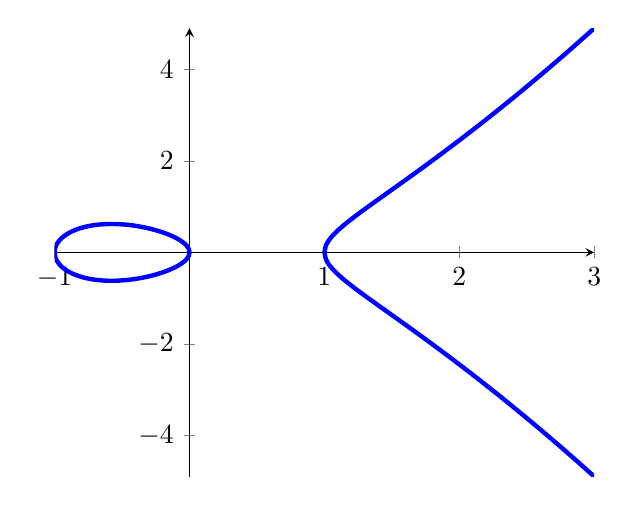
\begin{tikzpicture}
\begin{axis}[axis lines=middle]
\addplot[blue, ultra thick, samples=200, domain=1:3] (x, {(x^3-x)^(0.5)});
\addplot[blue, ultra thick, samples=200, domain=1:3
] (x, {-(x^3-x)^(0.5)});
\addplot[blue, ultra thick, samples=200, domain=-1:0] (x, {(x^3-x)^(0.5)});
\addplot[blue, ultra thick, samples=200, domain=-1:0] (x, {-(x^3-x)^(0.5)});
\end{axis}
\end{tikzpicture}
\end{figure}

If we instead think about complex solutions, we get something of the form of a torus minus a single point, with another rich geometric structure.

In $\C^3$, if $X = \{(x,y,z) \in \C^3 : x^3 + y^3 + z^3 = 1\}$, then $X$ contains 27 lines: $x = -\xi^m y, z = \xi^n$ for $i,j \in \{0,1,2\}$ gives 9 of them, and the other 18 come by rotating $x,y,z$ in this linear system.

In $\R^3$, consider the equation $1+x^3+y^3+z^3 = (1+x+y+z)^3$. %find pic of this

\section{Basic Setup}
Fix a field $K$. We define an \emph{affine n-space over K} to be $\mathbb{A}^n \coloneqq K^n$. Let $A \coloneqq K[x_1,x_2,\ldots,x_n]$ be the polynomial ring in $n$ variables over $K$, and let $S \subseteq A$ be a subset of $A$. We then define $\V(S)$, the \emph{vanishing locus of S} to be the set of all $n$-tuples $(a_1,\ldots,a_n) \in \mathbb{A}^n$ where $f(a_1,\ldots,a_n) = 0$ for all $f \in S$.

\begin{proposition}
\item
\begin{enumerate}
\item $\V(\{0\}) = \mathbb{A}^n$
\item $\V(A) = \emptyset$
\item $\V(S_1\cdot S_2) = \V(S_1) \cup \V(S_2)$, where $S_1\cdot S_2 = \{f_1\cdot f_2 : f_1 \in S_1, f_2 \in S_2\}$.
\item Let $I$ be an index set, $S_i \subseteq A$ for each $i \in I$. Then $\bigcap_{i \in I} \V(S_i) = \V(\bigcup_{i \in I} S_i)$
\end{enumerate}
\end{proposition}
\begin{proof} \textit{1., 2.} are obvious
\begin{enumerate}
\item If $p \in \V(S_1) \cup \V(S_2)$, then either $p \in \V(S_1)$ or $p \in \V(S_2)$. If $p \in \V(S_1)$, then $f_1(p) = 0$ for all $f_1 \in S_1$, and so $f_1(p)\cdot f_2(p) = 0$ for all $f_1 \in S_1, f_2 \in S_2$, so $p \in \V(S_1\cdot S_2)$, and similarly for if $p \in \V(S_2)$.

Conversely, suppose that $p \in \V(S_1\cdot S_2)$, and $p \notin \V(S_1)$. Then there is some $f_1 \in S_1$ with $f_1(p) \neq 0$. But $f_1(p)\cdot f_2(p) = 0$ for all $f_2 \in S_2$, and so $f_2(p) = 0$ for all $f_2 \in S_2)$, so $p \in \V(S_2)$.

\item If $p \in \V(S_i)$ for all $i \in I$, then $f_i(p) = 0$ for all $f_i \in S_i$, and so for all $f \in \bigcup_{i} S_i$, so $p \in \V(\bigcup_{i \in I}S_i)$.

Conversely, if $p \in \V(\bigcup_i S_i)$, then $f(p) = 0$ for all the polynomials in $\bigcup_i S_i$, and so $p \in \bigcap_i S_i$.
\end{enumerate}
\end{proof}
These four properties should remind you of the four axioms for a topology.

A subset of $\mathbb{A}^n$ is \emph{algebraic} if it of the form $\V(S)$ for some $S\subseteq A$. A \emph{Zariski open set} in $\mathbb{A}^n$ is a set of the form $\mathbb{A}^n \setminus \V(S)$ for some $S \subseteq \mathbb{A}^n$. This proposition tells us that the Zariski open sets define a topology on $\mathbb{A}^n$, called the \emph{Zariski topology}.

\underline{Examples:}
\begin{enumerate}
\item $K = \C$. The Zariski open (or closed) subsets of $\C^n = \mathbb{A}^n$ are in particular open (or closed) in the usual Euclidean sense, but not vice versa.
\item For any $K$, consider $\mathbb{A}^1, A = K[x], S \subseteq K[x]$. If $S$ has a non-zero element, then $\V(S)$ is finite. Thus the closed sets are the finite subsets of $\mathbb{A}^1$, and all of $\mathbb{A}^1$. The open sets are $\emptyset$ and all the co-finite sets (i.e. sets with finite complement).
\end{enumerate}

Recall that, if $A$ is any commutative ring with $S \subseteq A$ a subset, then the \emph{ideal generated by S} is the ideal $A \supseteq \angle{S} = \{\sum_{i=1}^q f_ig_i : q \geq 0, f_i \in S, g_i \in A\}$, or the smallest ideal of $A$ containing $S$.

\begin{lemma}
Let $S \subseteq A = K[x_1, \ldots, x_n]$. Then $\V(S) = \V(\angle{S})$.
\end{lemma}
\begin{proof}
If $p \in \V(S)$, then for $f_1, \ldots, f_q \in S; g_1, \ldots, g_q \in A$ we have:
\begin{align*}
\left(\sum_{i=1}^q f_ig_i\right)(p) = \sum_{i=1}^q f_i(p)g_i(p) = \sum_{i=1}^p 0\cdot g_i(p) = 0
\end{align*}
So $p \in \V(\angle{S})$, and so $\V(S)\subseteq \V(\angle{S})$. 

\hspace*{-1em}The other inclusion follows from the fact that $S \subseteq \angle{S}$, we must have $\V(\angle{S}) \subseteq \V(S)$.
\end{proof}

Let $X \subseteq \mathbb{A}^n$ be a subset. Define $I(X) \coloneqq \{f \in A : f(p) = 0 \;\forall p \in X\}$, the \emph{ideal of X}. Note that $I(X)$ is indeed an ideal, since if $f, g \in I(X)$ then $f+g \in I(X)$, and if $f \in I(X), g \in A$, then $f\cdot g \in I(X)$. Note that if $S_1\subseteq S_2 \subseteq A_1$, then $\V(S_2) \subseteq \V(S_1)$, and if $X_1 \subseteq X_2$, then $I(X_2) \subseteq I(X_1)$.

The \emph{radical} of an ideal $I \subset A$ is the set $\sqrt{I} \coloneqq \{x \in A: \exists n\in\N \st x^n \in I\}$. This is defined in general for any commutative ring $A$, not just polynomial rings.

\begin{lemma}
$\sqrt{I}$ is an ideal.
\end{lemma}
\begin{proof}
If $f, g \in \sqrt{I}$, there is $n, m$ such that $f^n, g^m \in I$. Then $(f+g)^{m+n} = \sum_{i=0}^{m+n} \binom{m+n}{i}f^i g^{m+n-i}$. Now for each term in this sum, either we have $i \geq n$ or $m+m-i\geq m$, and so one of these terms is in $I$. Hence by the closure rules for ideals, $(f+g)^{m+n} \in I$, so $f+g \in \sqrt{I}$. Given $f \in \sqrt{I}, g \in A$, we have $(fg)^n = f^n g^n$, and $f^n \in I \implies f^ng^n \in I$, so $fg \in \sqrt{I}$.
\end{proof}

\begin{proposition}
\item
\begin{enumerate}
\item If $X \subseteq \mathbb{A}^n$ is algebraic, then $\V(I(X)) = X$.
\item If $I \subseteq A$ is an ideal, then $I(\V(I)) \supseteq \sqrt{I}$.
\end{enumerate}
\end{proposition}
\begin{proof}
\item
\begin{enumerate}
\item Since $X$ is algebraic $X = \V(I)$ for some $I \subseteq A$. Certainly $I \subseteq I(X)$, and so $\V(I(X)) \subseteq \V(I) = X$. But $X \subseteq \V(I(X))$ trivially, and so $X = \V(I(X))$.

\item If $f \in \sqrt{I}$, then $f^n \in I$ for some $n$, and so $f^n$ vanishes on $\V(I)$, thus $f$ vanishes on $\V(I)$. Hence $f \in I(\V(I))$.
\end{enumerate}
\end{proof}
\begin{theorem}[Hilbert Nullstellensatz]
Let $K$ be algebraically closed. Then $I(\V(I)) = \sqrt{I}$.
\end{theorem}
\begin{proof}
Deferred until later.
\end{proof}

\hspace*{-1em}\underline{Example:} If $K = \R$, $I = \angle{x^2+y^2+1} \subseteq \R[x,y]$, then $\V(I) = \emptyset$, so $I(\V(I)) = \R[x,y] \neq \sqrt{I}$.

\hspace*{-1em}We define an \emph{affine (algebraic) variety} to be an algebraic subset of $\mathbb{A}^n$. Very often we can decompose affine varieties into smaller subsets. For instance, $\V(\angle{xy}) = + = - \cup | = \V(\angle{x}) \cup \V(\angle{y})$. If $Y \subseteq X$ is a non-empty closed subset, then we say $Y$ is \emph{irreducible} if whenever $Y = Y_1 \cup Y_2$ with $Y_1, Y_2$ closed, then either $Y_1 = Y$ or $Y_2 = Y$.  In the Euclidean topology on $\C^n$, the irreducible subsets are single points, but under the Zariski topology they are much more interesting. We will now turn to the question of identifying when an algebraic set is irreducible.

\begin{proposition}
If $X_1, X_2 \subseteq \mathbb{A}^n$, then $I(X_1 \cup X_2) = I(X_1) \cap I(X_2)$.
\end{proposition}
\begin{proof}
Since $X_1, X_2 \subseteq X_1 \cup X_2, I(X_1 \cup X_2) \subseteq I(X_1), I(X_2)$. Hence $I(X_1 \cup X_2) \subseteq I(X_1) \cap I(X_2)$.

Conversely, if $f \in I(X_1) \cap I(X_2)$, then $f$ vanishes on both $X_1$ and $X_2$, and so on all of the union. So $I(X_1) \cap I(X_2) \subseteq I(X_1 \cup X_2)$.
\end{proof}

Recall that an ideal $P \subseteq A$ of a commutative ring is said to be \emph{prime} if it is not the whole ring, and whenever $fg \in P$, either $f \in P$ or $g \in P$.

\begin{lemma}
Let $P \subseteq A$ be prime, and $I_1, \ldots, I_n \subseteq A$ be ideals. Suppose that $P \supseteq \bigcap_i I_i$. Then there is some $i$ such that $P \supseteq I_i$, and if equality holds in either then it holds in both.
\end{lemma}
\begin{proof}
Suppose $P \nsupseteq I_i$ for any $i$, so for all $i$ there is some $x_i \in I_i \setminus P$. Then $x = \prod_i x_i \in I_i$ for all $i$, so $x \in \bigcap_i I_i$ and hence $x \in P$. But then some $x_i \in P$ because $P$ is prime. \contr

If we have equality, then $P \subseteq I_i$ for all $i$, and by above there is some $i$ for which $P \supseteq I_i$, so $P = I_i$.
\end{proof}

\begin{proposition}
Let $K$ be algebraically closed. Then an algebraic set $X \subseteq \mathbb{A}^n$ is irreducible if and only if $I(X)$ is prime.
\end{proposition}
\begin{proof}
\item
\begin{itemize}
\item[$\implies$] If $f\cdot g \in I(X)$, then $X \subseteq \V(f\cdot g) = \V(f) \cup \V(g)$. So $X = (X \cap \V(f)) \cup (X \cap \V(g))$. Irreducibility implies that \textsc{wlog} $X = X\cap \V(f)$, i.e. $X \subseteq \V(f)$ as $\V(f), \V(g), X$ are closed. Then $f \in I(X)$, and so $I(X)$ is prime.

\item[$\impliedby$] If $P$ is prime with $\V(P) = X_1 \cup X_2$, $X_1, X_2$ closed. Then $I(X_1) \cap I(X_2) = I(X_1\cup X_2) = I(\V(P)) = \sqrt{P}$ by the Nullstellensatz. But if $f^n \in P$, then $f \in P$, and so $\sqrt{P} = P$. Hence $I(X_1)\cap I(X_2) = P$, and $P = I(X_1)$ or $I(X_2)$, so $\V(P) = X_1$ or $X_2$.
\end{itemize}
\end{proof}
So if $K$ is algebraically closed, then we have a one-to-one correspondence between algebraic subsets and radical ideals, and between irreducible algebraic subsets and prime ideals. This correspondence suggests that, just as prime ideals are the ``building blocks" of ideals, so too are irreducible varieties the building blocks of algebraic sets.

\begin{proposition}
Any algebraic set is a finite union of irreducible varieties.
\end{proposition}
\begin{proof}
Let $\mathcal{S}$ be the set of non-empty closed subsets of $\mathbb{A}^n$ which cannot be written as a finite union of irreducible subsets. Suppose $\mathcal{S} \neq \emptyset$. Then we claim $\mathcal{S}$ has a minimal element with respect to inclusion. 

If not, then there is an infinite descending chain of elements of $\mathcal{S}$, say, $X_1 \supsetneq X_2 \supsetneq \ldots$. If $I_j = I(X_j)$, then we get an \textit{ascending} chain of ideals $I_1 \subsetneq I_2 \subsetneq \ldots$. But since $K[x_1, \ldots, x_n]$ is Noetherian (proven in IB GRM), every ascending chain of ideals is eventually stationary. \contr.

Let $Y \in \mathcal{S}$ be a minimal element. Since $Y \in \mathcal{S}$, $Y$ is not irreducible, and so $Y = Y_1 \cup Y_2$, with $Y_1, Y_2 \neq Y$. Since $Y_i \subsetneq Y$ and $Y$ is minimal in $\mathcal{S}, Y_i \notin \mathcal{S}$, and so can be written as a finite union of irreducible closed subsets. But then $Y$ can also be written as a finite union of irreducible closed subsets.
\end{proof}

If $Y = \bigcup_{i=1}^n Y_i$, with $Y_i$ irreducible varieties, $Y_i \subseteq Y_j$ for $i \neq j$, then $Y_i, \ldots, Y_n$ are the \emph{irreducible components} of $Y$.

\hspace*{-1em}\underline{Example:} $\V(xy) = \V(x)\cup \V(y)$. Note that $\V(x)$ is irreducible because $(x)$ is a prime ideal in $K[x,y]$ - to see this observe $K[x,y]/(x) \cong K[y]$ is an integral domain. So the irreducible component of $\V(xy)$ are $\V(x)$ and $\V(y)$, or the two coordinate axes.

\begin{proposition}
The irreducible components of $Y$ are unique up to ordering.
\end{proposition}
\begin{proof}
Exercise.
\end{proof}

\hspace*{-1em}\underline{Example:} $A = K[x_1, \ldots, x_n]$ is a unique factorisation domain (UFD). If $f \in A\setminus\{0\}$, then $f$ is irreducible if and only if $(f)$ is prime. If instead, $f = f_1\ldots f_n$ is a factorisation into irreducible components, then $\V(f) = \V(f_1)\cup\ldots\cup \V(f_n)$ is the irreducible decomposition  of $\V(f)$.

For instance, $\V(y^2-x^3+x)$, the diagram on the first page of these notes, is irreducible.

\section{Regular and Rational Functions}
In algebraic geometry we are interested in polynomial functions, i.e. $f: \mathbb{A}^n \to K$ for some $f \in A = K[x_1, \ldots, x_n]$. Then, given $X \subseteq \mathbb{A}^n$ closed, we get $f|_X : X \to K$. Note that if there are $f,g \in A$ with $f|_X = g|_X$, then $(f-g)|_X = 0$, and so $f-g \in I(X)$.

Let $X \subseteq \mathbb{A}^n$ be an affine variety. We define the \emph{coordinate ring} of $X$ to be $A(X) \coloneqq A/I(X)$. The lecturer also uses the notation $K[X]$ to mean the same thing. I'm not sure why, but if you ever think we're doing some sort of polynomial ring in an affine variety, it's probably  because of this.

If $X$ is irreducible and $U \subseteq X$ is open, then a \emph{regular function} on $U$ is a function $f:U \to K$ such that, for every $p \in U$, there is an open neighbourhood $p \in V \subseteq U$, and functions $g, h \in A(X)$, with $h(q) \neq 0$ for all $q \in V$ and $f = g/h$ on $V$, i.e. everywhere in $U$ it is \textit{locally} a ratio of two polynomials.

\hspace*{-1em}\underline{Examples:}
\begin{enumerate}
\item $f \in A(X)$ induces $f|_U: U \to K$, which is $f/1$ on $U$ and so regular.
\item If $U \subseteq \mathbb{A}^1$, $U = \mathbb{A}^1 \setminus\{0\}$. Then $g(x)/x^n$ is a regular function on $U$ for any polynomial $g$.
\end{enumerate}

We write for $U \subseteq X$ open, $\mathcal{O}_X(U) \coloneqq \{f:U \to K: f\text{ a regular function}\}$. Note that $\mathcal{O}_X(U)$ is a ring, i.e. sums, products, and differences of regular functions are regular. $\mathcal{O}_X(U)$ is also a $K$-algebra, so we can multiply by scalars in $K$.

\begin{lemma}
$\mathcal{O}_X(X) = A(X)$ if $K$ is algebraically closed.
\end{lemma}
\begin{proof}
Deferred until after Hilbert's Nullstellensatz.
\end{proof}

Recall that, if $A$ is an integral domain, then we define the \emph{field of fractions} of $A$ to be $\Big\{\frac{f}{g} : f \in A, g \in A \setminus\{0\}\Big\}/\thicksim$, with $\frac{f}{g} \thicksim \frac{f'}{g'}$ if $fg' = f'g$. This is, as the name would suggest, a field.

If $X \subseteq \mathbb{A}^n$ is an irreducible variety, then we define the \emph{function field} of $X$ to be the field of fractions of $A(X)$. We denote this $K(X)$. Note that $A(X)$ is an integral domain if and only if $X$ is irreducible. Then $f \in K(X)$ can be written as $f=\frac{g}{h}$ for $g,h \in A(X)$, and this is a regular function on $X \setminus \V(h)$.

\section{Morphisms}
A map $f:X \to Y$ between affine varieties is a \emph{morphism} if:
\begin{enumerate}
\item $f$ is continuous in the Zariski topology (i.e. the induced topologies on $X$ and $Y$)
\item For all open $V \subseteq Y$ and for any regular function $\varphi: V \to K$, the map $\varphi \circ f: f^{-1}(V) \to K$ is also regular.
\end{enumerate}
The lecturer appreciates that this is a conceptually difficult definition, but has no idea how to make it clearer.

If $f:X \to Y$ is a morphism, then for any $\varphi \in A(Y), \varphi\circ f$ is a regular function on $X$, and hence $\varphi \circ f \in A(X)$ by \textbf{2.1}. This defines a map $f^{\#}:A(Y) \to A(X); \varphi \mapsto \varphi\circ f$.

Note that $f^{\#}$ is a $K$-algebra homomorphism:
\begin{itemize}
\item $f^{\#}(\varphi_1+\varphi_2) = (\varphi_1+\varphi_2)\circ f = \varphi_1 \circ f + \varphi_2 \circ f = f^{\#}(\varphi_1) + f^{\#}(\varphi_2)$.
\item $f^{\#}(\varphi_1\cdot\varphi_2) = f^{\#}(\varphi_1)f^{\#}(\varphi)$
\item For $a \in K$, $f^{\#}(a \cdot \varphi) = f^{\#}(a)f^{\#}(\varphi) = af^{\#}(\varphi)$
\end{itemize}

\begin{theorem}
There is a one-to-one correspondence between morphisms $f:X \to Y$ of affine varieties and $K$-algebra homomorphisms $f^{\#}:A(Y)\to A(X)$.
\end{theorem}
\begin{proof}
We've seen how to get $f^{\#}$ from $f$. So now suppose we have $f^{\#}:A(Y) \to A(X)$ a $K$-algebra homomorphism given. Suppose $X \subseteq \mathbb{A}^n, Y \subseteq \mathbb{A}^m$. Then:
\begin{align*}
A(X) = \frac{K[x_1, \ldots, x_n]}{I(X)}\hspace{7em}A(Y) = \frac{K[y_1, \ldots, y_m]}{I(Y)}
\end{align*}
Let $\bar{y_i}$ be the element of $A(Y)$ represented by $y_i$, and let $f_i = f^{\#}(\bar{y_i}) \in A(X)$.

Then let $f: X \to \mathbb{A}^m$ be given by $f(p) = (f_1(p),\ldots, f_m(p))$. We claim that the image of $f$ lies in $Y$.

We have the maps $K[y_1, \ldots, y_m] \xrightarrow{\text{quotient map}} A(Y) \xrightarrow{f^{\#}} A(X)$ given by $y_i \mapsto \bar{y_i} \mapsto f_i$, and so $g \mapsto g(f_1, \ldots, f_m)$.

Then since $g \in I(Y)$, we have $g(f_1, \ldots, f_m) = 0$ in $A(X)$, and so in particular, evaluating at $p$, we get $g(f_1(p), \ldots, f_m(p)) = 0$ as desired. Note that if $\varphi \in A(Y)$ we can write $\varphi = \bar{g}$ for some $g \in K[y_1, \ldots, y_m]$, and then $f^{\#}(\varphi) = g(f_1, \ldots, f_m) \in A(X)$. Hence $f$ is a map from $X$ to $Y$.

Next, we must show that $f:X \to Y$ is a morphism.

For continuity, we show that if $Z \subseteq Y$ is closed, then $f^{-1}(Z) \subseteq X$ is closed. For this, note $I(Z) \supseteq I(Y)$, and write $\overline{I(Z)}$ for the image $I(Z)/I(Y)$ in $A(Y)$. This is the ideal of regular functions on $Y$ vanishing on $Z$.
\begin{align*}
\V(f^{\#}(\overline{I(Z)})) &= \{p \in X : g(p) = 0 \forall g \in f^{\#}(\overline{I(Z)})) \subseteq A(X)\}\\
&= \{p \in X : (h\circ f)(p) = 0 \forall h \in \overline{I(Z)}\}\\
&= \{p \in X : f(p) \in \V(\overline{I(Z)})\}\\
&= \{p \in X : f(p) \in Z \}\\
&= f^{-1}(Z)
\end{align*}
If $I$ denotes the inverse image of $f^{\#}(I(Z))$ under the quotient map $K[x_1, \ldots, x_n] \to A(X)$. Then $\V(I) = \V(f^{\#}(\overline{I(Z)}))$, and in particular $f^{-1}(z)$ is closed.

If $\varphi \in \mathcal{O}_Y(U)$, i.e. $\varphi:U \to K$ is regular, we need to show that $\varphi \circ f: f^{-1}(U) \to K$ is regular. Let $p \in f^{-1}(U)$. Then there exists a neighbourhood $V \subseteq U$ of $f(p)$ on which $\varphi|_V = \frac{g}{h}$ for $g, h \in A(Y)$ with $h$ non-vanishing on $V$.

Then $(\varphi \circ f)|_{f^{-1}(V)} = \varphi|_V \circ f = \frac{g}{h}\circ f = \frac{g\circ f}{h\circ f} = \frac{f^{\#}(g)}{f^{\#}(h)}$. Here, $f^{\#}(g). f^{\#}(h) \in A(X)$, and $f^{\#}(h) = h \circ f$ does not vanish on $f^{-1}(V)$. Hence $\varphi\circ f$ is regular as desired, and hence a morphism.
\end{proof}

The moral of this notationally heavy proof is that a morphism $f: X\to Y$ is given by a choice of polynomials $f_1, \ldots, f_n \in K[x_1, \ldots, x_n]$ such that $f(p) = (f_1(p), \ldots, f_m(p)) \in Y$ for all $p \in X$.

\hspace*{-1em}\underline{Example:} $f: \mathbb{A}^1 \to \mathbb{A}^2; t \mapsto (t, t^2)$, so that $f_1(t) = t, f_2(t) = t^2$. Then $f^{\#}$ is a homomorphism of rings from $K[y_1, y_2] \to K[t]$, with $f^{\#}(y_1) = t, f^{\#}(y_2) = t^2$. Note that $y_1^2-y_2 \in \ker f^{\#}$, so in fact we have a $K$-algebra homomorphism, $f^{\#}:K[y_1, y_2]/(y_1^2-y_2) \to K[t]$, inducing a morphism $f:\mathbb{A}^1 \to Y = \V(y_1^2-y_2)$, a parabola.

We say $X$ and $Y$ as affine varieties are \emph{isomorphic} if there is $f:X \to Y, g:Y \to X$ both morphisms with $f\circ g = \id_Y, g \circ f = \id_X$.

\begin{corollary}
$X$ and $Y$ are isomorphic if and only if $A(X)$ and $A(Y)$ are isomorphic as $K$-algebras.
\end{corollary}

\section{Projective Space}
Consider the two lines $\ell_1 = \V(x), \ell_2 = \V((1+1/t)x + 1)$, for $t$ some parameter in $K$. Then the intersection $\ell_1 \cap \ell_2$ is is a single point for $t \neq \infty$. However, at $t = \infty$ the lines are parallel, and so we have lost this intersection. We think of this as being a failure of compactness, and introduce the idea of projective space to restore this compactness.

Let $U$ be a vector space of dimension $n+1$ over $K$. Then the \emph{projectivization} of $U$, $\P(U)$ is the set of all 1-dimensional subspaces of $U$. We will write $\P^n \coloneqq \P(K^{n+1})$.

For example, $\P^1 = \P(K^2) = \{$nonzero vectors in $K^2\}/$scaling action of $K^{\ast}$, where by this scaling action we identify $(1,1) \thicksim (2,2) \thicksim (-1,-1)$. More formally, this is the quotient space $\left(\mathbb{A}_K^2\setminus\{0\}\right)/ \thicksim$ where $(z_0,z_1) \thicksim (\lambda z_0, \lambda z_1)$ for $\lambda \in K^{\ast}$, so that the equivalence classes of $\thicksim$ are straight lines through the origin.

Why does this ``compactify" $\mathbb{A}^1$? Consider the subset of $\P^1$ given by $\{(z_0, z_1) \in \P^1 : z_0 \neq 0\} = \{(1, z_1/z_0) : z_0 \neq 0, z_1 \in K\}$, using the equivalence relation. But this is isomorphic to $\mathbb{A}^1$, by picking $z_1 = z_0 k$ for $k \in K$, so $\P^1$ contains all the information about $\mathbb{A}^1$ by encoding each element in $\mathbb{A}^1$ as the gradient of a line in $\mathbb{A}^2$, together with some missing information, where $z_0 = 0$. In the $\mathbb{A}^1$ ``view" of $\P^1$, this point is the point at infinity, which seems special or distinguished in some way, but we view it as a line in $\mathbb{A}^2$, it is simply another straight line through the origin $\{(0,t) : t \in K\}$.

We can think of $\P^1$ in another way - if we draw in the unit circle centered on the origin in the $\mathbb{A}^2$ view of $\P^1$, we see we have a bijection between the straight lines through the origin (elements of $\P^1$ as defined) and pairs of antipodal points on the unit circle. So we can also view $\P^1$ as the unit circle in $\mathbb{A}^2$ with antipodal points identified.

\begin{figure}[H]
\centering
\begin{subfigure}{.5\textwidth}
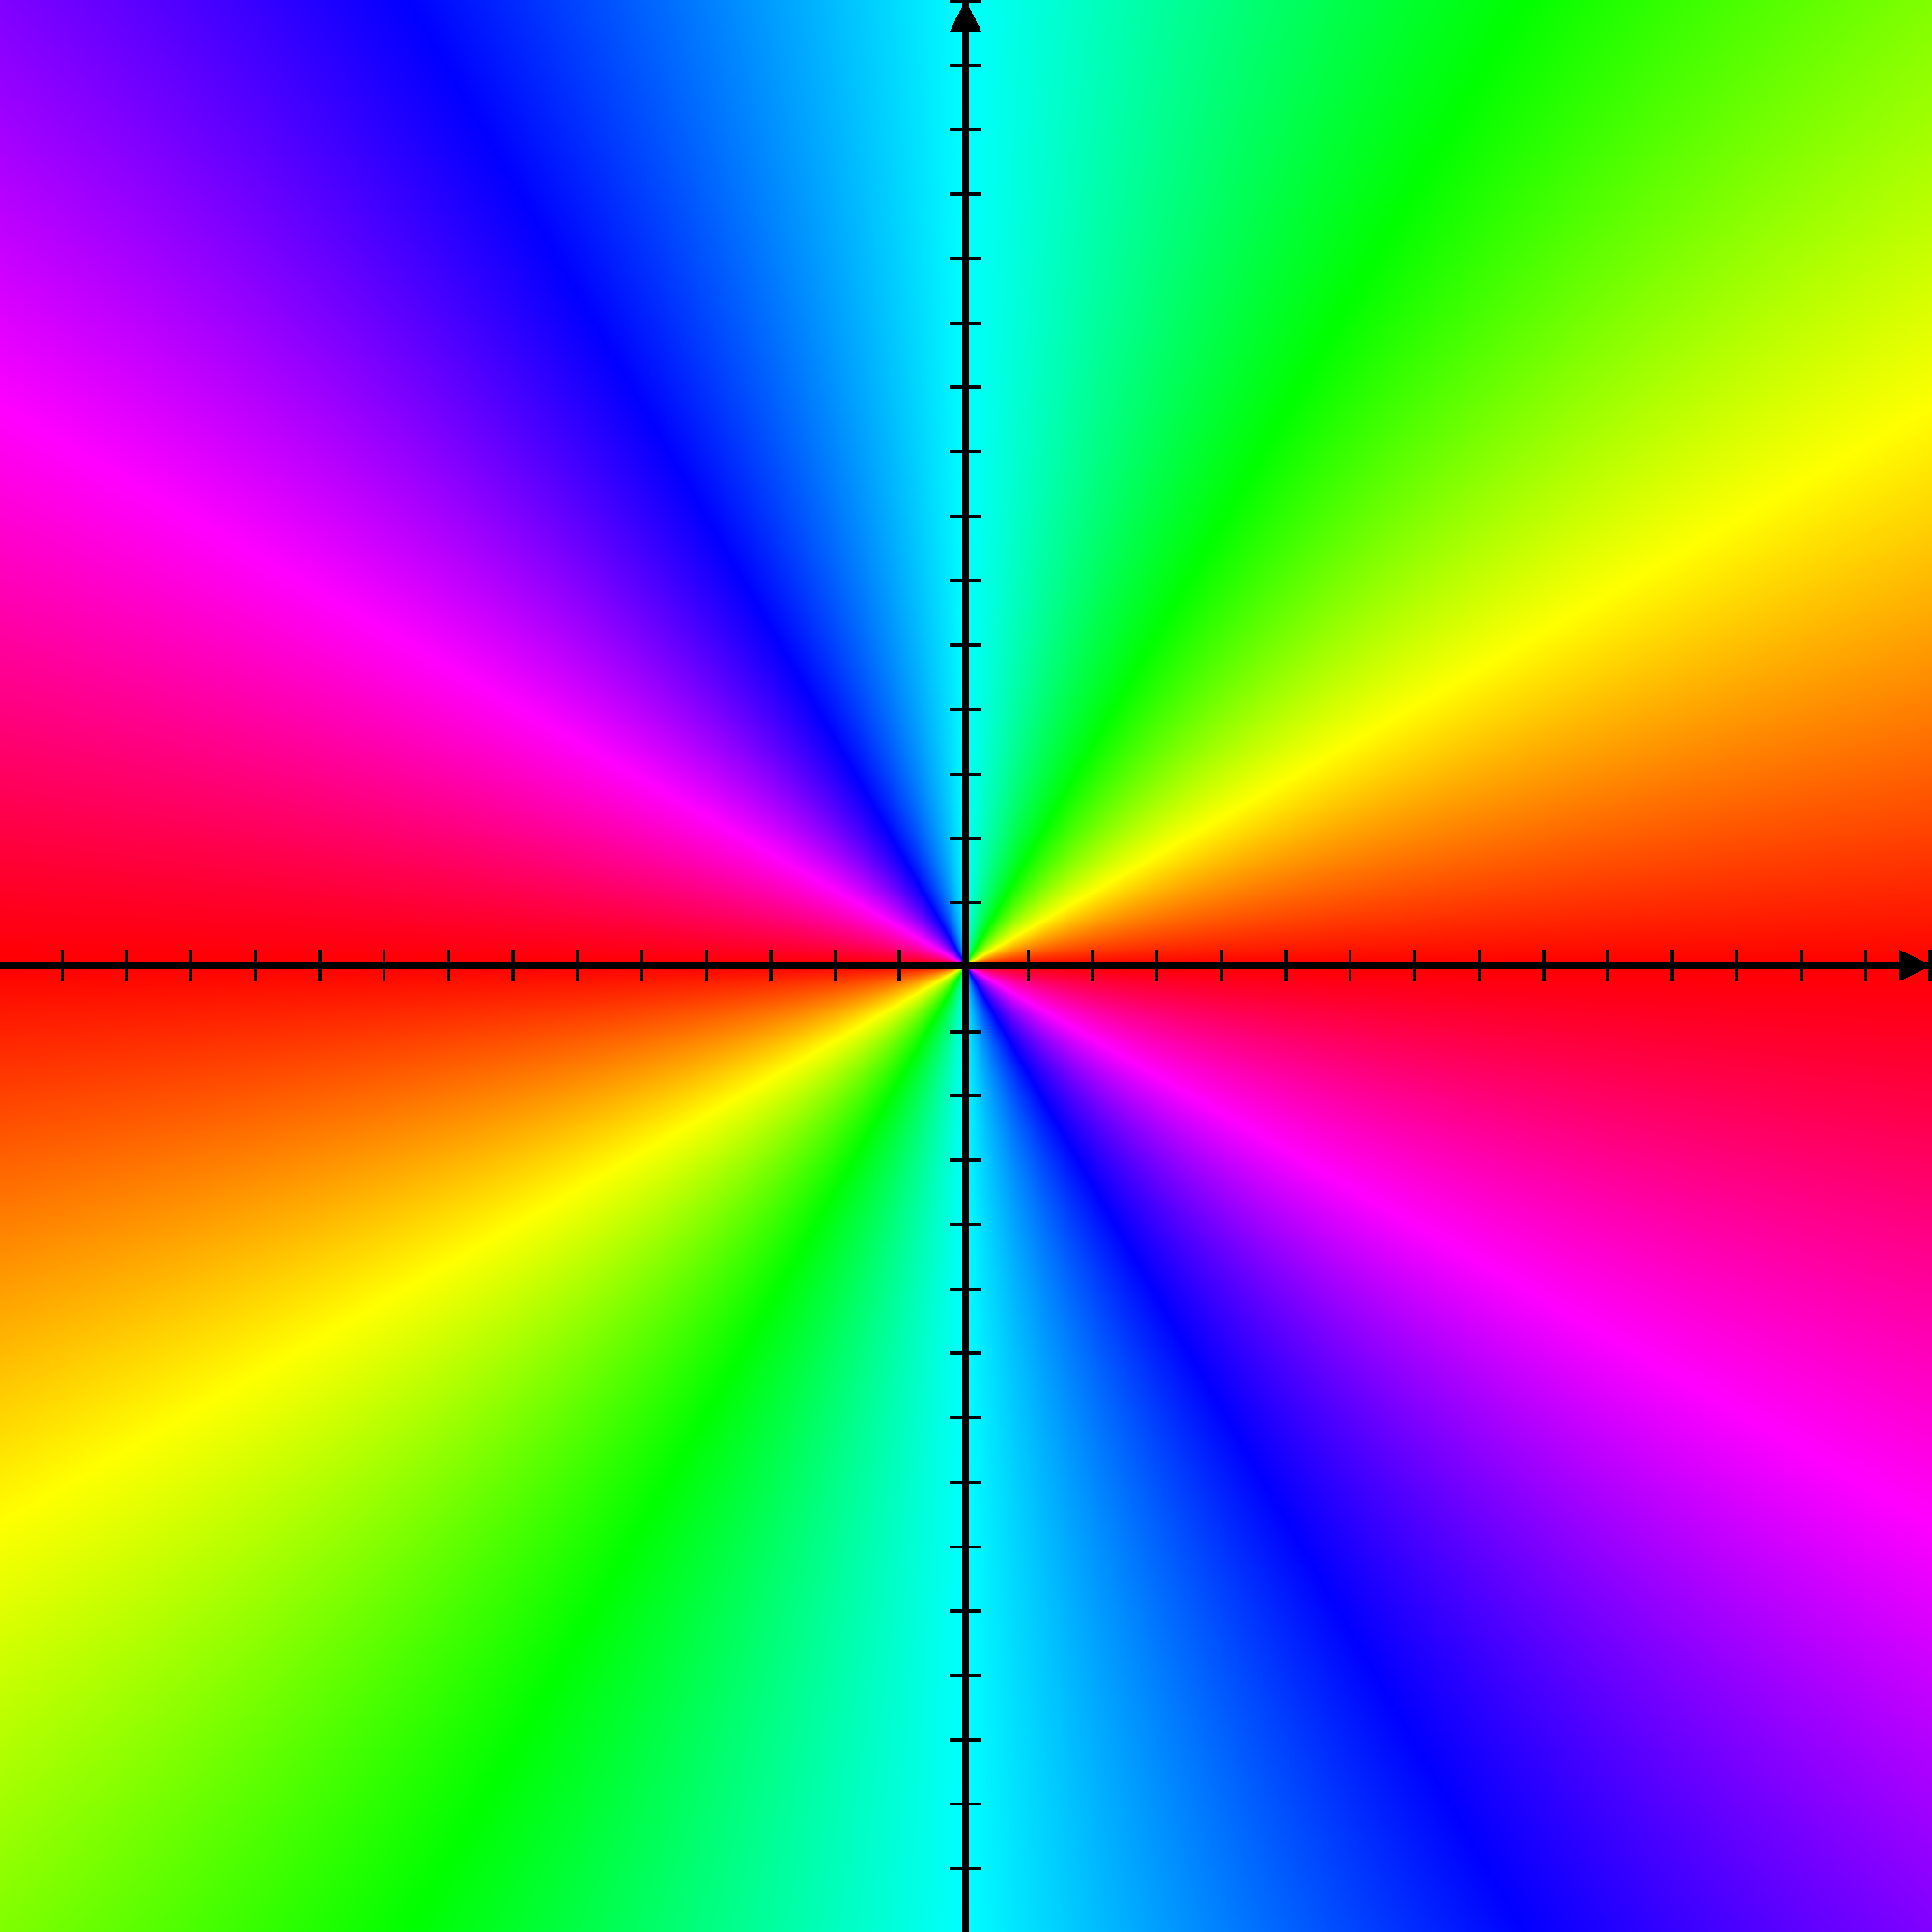
\includegraphics[scale=.1]{plane.png}
\caption{$\P^1$ as the straight lines in $\A^2$, so that points of the same colour are identified}
\end{subfigure}\\
\begin{subfigure}{.4\textwidth}

\includegraphics[scale=.1]{line.png}
\caption{$\P^1$ as the corresponding points in $\A^1$, i.e. the gradients of lines. Note the point at infinity}
\end{subfigure}\hfill
\begin{subfigure}{.4\textwidth}

\includegraphics[scale=.1]{circle.png}
\caption{$\P^1$ as the points on a circle, with antipodal points identified (points of the same colour)}
\end{subfigure}
\end{figure}

For $\P^2_K$, consider $\P^2_K \supseteq \mathcal{U}_0 = \{(z_0,z_1,z_2):z_0 \neq 0\} = \{(1,z_1/z_0,z_2/z_0):z_0\neq 0\} \cong \mathbb{A}_K^2$. The missing stuff at infinity is $\P^2 \setminus \mathcal{U}_0 = \{(0,z_1, z_2): (z_1,z_2) \neq (0,0)\}/$scaling $ \cong \P^1$. Similarly as in the $\P^1$, we can think of $\P^2$ as being a sphere with antipodal points identified.

In general, in $\P^n$ with \emph{homogeneous coordinates} $[z_0, \ldots, z_n]$, (where the square brackets indicates that we are working with an equivalence class of coordinates)\footnote{Also used in literature are the notations $(z_0:z_1:\ldots:z_n)$ or $[z_0:z_1:\ldots:z_n]$} we have subsets $\mathcal{U}_i = \{(z_0, \ldots, z_n):z_i \neq 0\}\cong \mathbb{A}_k^n$ for $0\leq i\leq n$, we have $\P_K^n \setminus \mathcal{U}_i = \P_K^{n-1}$.

\subsection{Projective Varieties}
We want to extend our idea of an affine variety to some sort of ``projective variety" in projective space. The idea of polynomial function in $z_0, \ldots, z_n$ is not well defined on points in projective space, because of the scaling that we have quotiented out by. For instance, take the polynomial $f=z_0 + 1$ as a function on $\P_K^2$. We expect to obtain values in $K$ for $f(p)$ where $p \in \P_K^2$. But $(1,0,0) \thicksim (-1,0,0)$ are equivalent in $\P_K^2$, and $f(1,0,0) = 2, f(-1,0,0) = 0$, so $f$ is not well defined on $\P^2_K$.

It's not so much a problem that the value of the polynomial isn't well defined, and we never really used this property in the affine case. We only cared that the points where it was zero, $\V(f)$, was well defined. Similarly, in the projective case, we can see that the polynomial will have a well defined zero set when $f(A p) = B f(p)$ for fixed constants $A, B$ independent of $p$. Plugging this into the definition of a polynomial, we obtain the following criterion:

A polynomial $f \in K[z_0, \ldots, z_n]$ is \emph{homogeneous of degree d} if $f(\lambda p) = \lambda^d f(p)$ for all $\lambda \in K^{\ast}, p \in \mathbb{A}_K^n$. Equivalently, if the total degree of every term is $d$.
\begin{itemize}
\item $z_0^2 + 2z_1z_2 + 8z_2^2$ is homogeneous, as the total degree of each term is 2.
\item $z_0 + z_1^2 + 2z_2^3 + 1$ is not homogeneous, as the terms have total degree 1, 2, 3, 0 respectively.
\end{itemize}

A \emph{projective hypersurface} in $\P_K^n$ is the vanishing set $\V(f)\subseteq \P_K^n$ for a $f$ a homogeneous polynomial in $K[z_0, \ldots, z_n]$. This \textit{is} well defined, since $f$ is homogeneous.

An ideal in $K[z_0, \ldots, z_n]$ is \emph{homogeneous} if it is generated by homogeneous polynomials, not necessarily of the same degree.
\begin{lemma}
The following two conditions are equivalent for an ideal $I \subseteq K[z_0, \ldots, z_n]$:
\begin{enumerate}
\item $I$ is homogeneous.
\item If $f \in I$, then every constituent in $f$ of degree $r$, denoted $f_{[r]}$ also lies in $I$.
\end{enumerate}
\end{lemma}
By this we mean that every polynomial $f \in K[z_0, \ldots, z_n]$ can be written as a sum $\sum_{r=0}^d f_{[r]}$ where $f_{[r]}$ is homogeneous of degree $r$. For example:
\begin{align*}
z_0 + 2z_1^2 + z_0z_2 + z_2^3 + 3z_2 = \underbrace{0}_{f_{[0]}} + \underbrace{z_0 + 3z_2}_{f_{[1]}} + \underbrace{2z_1^2 + z_0z_2}_{f_{[2]}} + \underbrace{z_2^3}_{f_{[3]}}
\end{align*}
\begin{proof}
\textit{2.}$\implies$\textit{1.} is immediate, since $I$ is generated by the constituent parts of all of its polynomials, which are all homogeneous.

For the other direction, let $I = \angle{f_j}$ where $f_j$ is homogeneous of degree $d_j$. Then for $f \in I$, $f = \sum_j h_j f_j$ where $h_j$ is arbitrary and $f_j$ is homogeneous.

Now split $h_j$ into its constituent homogeneous pieces, so that $h_j = \sum_r h_{j[r]}$, a sum of terms of degree $r$. Then $f_{[r]} = \sum h_{j[d_j-r]} f_{j[r]}$. Now $f_{j[r]} = f_j$ if $r = d_j$, and $0$ otherwise since $f_j$ is homogeneous, so $f_{j[r]} \in I$. Then $f_{[r]}$ is a sum of terms $hg$ for $g \in I, h \in K[z_0, \ldots, z_n]$, and so $f_{[r]} \in I$ as required.
\end{proof}

Let $I \subseteq K[z_0, \ldots, z_n]$ be a homogeneous ideal. Then the associated \emph{projective variety} is $\V(I) = \{P \in \P^n_K : f(P) = 0 \forall f \in I\}$, which by the previous lemma is the same as saying $f(P)$ vanishes for every homogeneous $f \in I$. Projective space then inherits a Zariski topology in three ways:
\begin{enumerate}
\item Closed sets are given by $\V(I)$ for $I \subseteq K[z_0, \ldots, z_n]$ homogeneous.
\item $\P^n_K$ is covered by $n+1$ open sets $\mathcal{U}_i = \P^n_K \setminus \{z_i = 0\}$, each in bijection with $\mathbb{A}^n_K$ which has a Zariski topology, so each $\mathcal{U}_i$ has a Zariski topology. Now declare a subset $C \subseteq \P^n_K$ closed if and only if $C \cap \mathcal{U}_i = 0$ for all $i$.
\item We describe $\P^n_K = \big(\mathbb{A}^{n+1}_K \setminus \{(0,0,0)\}\big)/\thicksim$, and then inherit the topology as a quotient topology of the Zariski topology on $\mathbb{A}_K^n$.
\end{enumerate}
\begin{lemma}
These three topologies are equivalent.
\end{lemma}
\begin{proof}
Exercise for a topology course.
\end{proof}
We call this topology the \emph{Zariski topology on $\P^n_K$}.

Notice that, via description 3, $\P_\C^n$ is a compact topological space and even Hausdorff with respect to the second ``Euclidean" topology, by observing it is a quotient of a unit hypersphere. We will often draw diagrams of projective space using this Euclidean topology, although this structure cannot be detected using the Zariski topology. The Zariski topology is weird, so we don't draw diagrams using it.

Let $\mathcal{U}_0 \subseteq \P_K^n$ be the locus where $Z_0 \neq 0$, and let $X = \V(f)$ for some $f \in K[\mathbf{z}]$. Then $X \cap \mathcal{U}_0$ can be described by $\V\Big(f\big(1, \frac{z_1}{z_0}, \ldots, \frac{z_n}{z_0}\big)\Big)$. As a consequence, every projective variety $X \subseteq \P_K^n$ is a union of $n+1$ affine varieties, as $\bigcup_{i=0}^n X \cap \mathcal{U}_i$.

A projective variety $X \subseteq \P_K^n$ is irreducible if $X$ cannot be written as a union $X = X_1 \cup X_2$ with the $X_i$ nonempty proper subvarieties.

Let $X \subseteq \P_K^n$ be a projective variety. Then the \emph{homogeneous ideal of X} $I^h(X)$ is the ideal generated by all homogeneous polynomials vanishing on $X$.

\begin{lemma}
$X$ is irreducible if and only if $I^h(X)$ is a prime ideal.
\end{lemma}
\begin{proof}
This is the same as in the affine case, observing the following fact: If $J \subseteq K[\mathbf{z}]$ is homogeneous and non-prime then there exist $F, G \in K[\mathbf{z}]$ homogeneous with $FG \in J$ but neither $F$ nor $G$ in $J$.
\end{proof}
Hence, via our discussion in the affine case, every projective variety has a unique irreducible component decomposition. Consider the ideal $I \subseteq K[\mathbf{z}]$ given by $I = \angle{z_0, \ldots z_n}$. Then $\V(I) = \emptyset$ in $\P_K^n$ as $(0,\ldots, 0) \notin \P^n_K$.

\begin{theorem}[Projective Nullstellensatz]
\item
\begin{enumerate}
\item If $I \subseteq K[\mathbf{z}]$ is a homogeneous ideal such that $\V(I) = \emptyset \subseteq \P^n_K$, then $I \supseteq \angle{z_0^m: \ldots: z_n^m}$ for some $m > 0$.

\item If $X = \V(I)$ with $I$ homogeneous, then $I^h(X) = \sqrt{I}$.
\end{enumerate}
\end{theorem}
\begin{proof}
Essentially the same as the affine case, which will come later.
\end{proof}

If $X \subseteq \P^n_K$ is a projective variety, then every algebraic function $X \to \C$ is constant, by Liouville's theorem. This is why we introduce the idea of rational functions.

\subsection{Rational Functions}
Let $X \subseteq \P_K^n$ be an irreducible projective variety. Then we define the \emph{function field} $K(X)  = \left\{\frac{f}{g} : f,g\text{ homogeneous of same degree }, g \in I^h (X)\right\} / \thicksim$, where $\frac{f_1}{g_1} \thicksim \frac{f_2}{g_2} \iff f_1g_2-g_1f_2 \in I^h(X)$.

Note that these ratios of polynomials of the same degree are well defined on projective space - when the scaling term of $\lambda^d$ comes out in the numerator and the denominator it cancels, so that $\frac{f(\lambda z)}{g(\lambda z)} = \frac{f(z)}{g(z)}$.

We need to check that $K(X)$ is well defined, i.e. that the equivalence relation $\thicksim$ is indeed an equivalence relation, and also that $K(X)$ is a field. The first of these requires that $I^h(X)$ is prime.

The set of degree $d$ homogeneous polynomials in variables is a $K$-vector space denoted $\mathcal{O}_{\P^n}(d)$, where $\dim_K \mathcal{O}_{\P^n}(d) = |\{\text{monomials of degree $d$ in $z_0, \ldots, z_n$}\}| = \binom{n+d}{d}$.

We can think of $(n+1)\times(n+1)$ matrices (i.e. elements of $GL(n+1,K)$) as changing coordinates in $K^{n+1}$, and inducing a change of homogeneous coordinates on $\P^n_K$. These changes of coordinates are unique up to scaling, so we have the group of matrices corresponding to changes of homogeneous coordinates given by $\P GL(n+1, K) \cong GL(n+1, K)/\text{scaling}$.

For example, $\P GL(2, \C)$ is the group of M\"obius transformations on $\P^1_\C$.

Let $p_1, \ldots, p_{n+2}$ be a set of points in $\P^n_K$ such that no $n+1$ of these lie in a hyperplane $\V(f)$ for $f \in \mathcal{O}_{\P^n}(1)$. Then there exists a change of coordinates $\phi : \P^n_K \to \P^n_K$ such that:
\begin{align*}
\phi(p_1) &= [1:0:\ldots:0]\\
\phi(p_2) &= [0:1:\ldots:0]\\
&\vdots\\
\phi(p_{n+1}) &= [0:0:\ldots:1]\\
\phi(p_{n+2}) &= [1:1:\ldots:1]
\end{align*}
This is a simple exercise in linear algebra. Hence we can see that $\P GL(n+1, K)$ acts transitively on the set of collections of $n+2$ points in general position. This follows by choosing an appropriate basis of $K^{n+1}$.

\begin{proposition}
Let $F \in \mathcal{O}_{\P^2} (d)$ and assume that $F$ is irreducible. Let $c = \V(F)$ and $\ell \subseteq \P^2$ be a line (i.e. $\ell = \V(G)$ for $G \in \mathcal{O}_{\P^2}(1)$. Then $\#\ell \cap c \leq d$, and in fact there exist positive integers $m_p(c, \ell)$ for $p \in c\cap \ell$ such that $\sum_{p \in c\cap\ell} m_p(c, \ell) = d$.
\end{proposition}
\begin{proof}
Choose coordinates $z_0, z_1, z_2$ on $\P^2_K$ such that the following things hold:
\begin{itemize}
\item $\ell = \V(z_2)$
\item $[0:1:0] \notin c$
\end{itemize}
This implies that $c \cap \ell \subseteq \P_K^2 \setminus \{z_0 = 0\}$. But this is $\P_K^2 \setminus \mathcal{U}_0 \cong \mathbb{A}^2_K$, and so we can work in the affine case.

If we choose $x = \frac{z_1}{z_0}, y = \frac{z_2}{z_0}$, then $c \cap \{z_0 \neq 0\} = \V(f(x_y)), f(x,y) = F(1,x,y)$. Now, since $[0:1:0] \notin c$, $f(x,y)$ has degree $d$ in the $x$ variable. Hence $c\cap \ell = \{f(x,y) = 0\}$, and the result follows by the fundamental theorem of algebra, where the $m_p(c, \ell)$ are the multiplicities of the roots.
\end{proof}
This implies that any two distinct lines in $\P^2_K$ intersect at a point.

in fact, if $C = \V(F_1), D = \V(F_2)$ for $F_i \in \mathcal{O}_{\P^2}(d_i)$ irreducible, then $C \cap D$ is $d_1d_2$ points counted with multiplicity (Bezout's theorem).

\begin{lemma}
Let $F$ and $G$ be homogeneous polynomials that are coprime, with $\deg(F), \deg(G) \leq 2$. Then
\begin{align*}
\# \V(F) \cap \V(G) \leq \deg(F)\deg(G)
\end{align*}
\end{lemma}
\begin{proof}
Omitted, similar to proposition above.
\end{proof}
\begin{proposition}
Let $p_1, \ldots, p_5 \in \P^2_K$, where no three lie on a line. Then there exists a unique \emph{conic curve} $C = \V(F), F \in \mathcal{O}_{\P^2}(2)$ passing through $p_1, \ldots, p_5$. Moreover, $C$ is irreducible.
\end{proposition}
\begin{proof}
Suppose there existed two conics $C_1, C_2$ through the points. Then they intersect at $>4$ points, so they contradict the lemma above. But why does such a conic exist?

Any conic is given by $\V(a_1z_0^2+a_2z_1^2+a_3z_2^2+a_4z_1z_2+a_5z_0z_1+a_6z_0z_2) = \V(F)$ where $(a_1, \ldots, a_6) \in K^2\setminus \{\mathbf{0}\}$. Now each condition that $\V(p_i) = 0$ is a linear condition in the coefficients $a_1, \ldots, a_6$. Linear algebra guarantees a one dimensional solution, but they are all multiples of each other so we get a unique irreducible polynomial $F$, and so $C$ exists and is irreducible.
\end{proof}
If $F \in \mathcal{O}_{\P^2}(3)$, $\V(F)$ is usually called an elliptic curves.

\subsection{The Rational Normal Curve, or the Twisted Cubic, and Other Short Stories}
Suppose we have a map from $\P^1 \to \P^3$, where $[x_0:x_1]\mapsto [x_0^3:x_0^2x_1:x_0x_1^2:x_2^3]$. We call this map the \emph{twisted cubic}. In the affine patch $\{x_0 \neq 0\}$, this is given by $\A^1 \to \A^3; t \mapsto (t, t^2, t^3)$, the \emph{rational normal curve}. The image of this map is an algebraic variety with equations
\begin{align}
z_0z_2 - z_1^2 &= 0\\
z_0z_3 - z_1z_2 &= 0\\
z_1z_3 - z_2^2 &= 0
\end{align}
Take another map from $\P^1 \times \P^1 \to \P^3; ([x_0:x_1], [y_0:y_1]) \mapsto [x_0y_0:x_0y_1:x_1y_0:x_1y_1]$ - it is easy to check this is well defined. This map in injective onto $\P^3$, and its image is precisely the vanishing locus of equation (2) - this can be checked by considering the affine patches where the map becomes a morphism $\mathbb{A}^1 \to \mathbb{A}^3$. The vanishing locus of $(z_0z_3 - z_1z_2)$ endows $\P^1 \times \P^1$ with the structure of a projective algebraic variety.

We call $\Sigma_{1,1} \subseteq \P^3$ the image of $\P^1 \times \P^1$ under this map.
\begin{enumerate}
\item $\Sigma_{1,1}$ contains a family of lines $\{L_t\}_{t \in \P^1}$ such that $L_t \cap L_{t'} = \emptyset$ if $t \neq t'$.
\item There is in fact another family $\{M_t\}_{t \in \P^1}$ of disjoint lines such that $M_t \cap L_{t'} = \ast$, some single point, for all $t, t' \in \P^1$.
\end{enumerate}
We get these lines by fixing one coordinate of $\P^1$ and letting the other vary - in this way injectivity gives the families of lines.

If $X$ is an irreducible projective variety, then its \emph{field of rational functions} is given by
\begin{align*}
K(X) &= \left\{ \frac{F}{G} : F, G \in K[\mathbf{z}] \text{ homogeneous of same degree, } G \notin I^h(X)\right\}/\thicksim\\
\frac{F_1}{G_1} \thicksim \frac{F_2}{G_2} & \iff F_1G_2 - F_2G_2 \in I^h(X)
\end{align*}
However, computing $K(X)$ is a pain - checking if things are members of ideals is a pain to do. Instead, we can compute $K(X)$ via the affine case.

\subsection{Projective Closures}
If $f \in K[z_1, \ldots, z_n]$, then $\V(f) \subseteq \A^n_k.$ If we consider $\A_K^n=\P_K^n\setminus \{z_0 =0\}$, we can consider the Zariski closure of $\V(f)$ in $\P^n_K$. To do this, we need to \emph{homogenize} our polynomials. Say $d$ is the maximum degree of a variable $z_i$ appearing in $f$. Then $f^h \coloneqq z_0^d f(z_1/z_0, \ldots, z_n/z_0)$. For example, if $f(z_1,z_2) = z_1^3 + z_1z_2, f^h(z_0,z_1,z_2) = z_1^3 + z_0z_1z_2$.

Similarly for an ideal $I \subseteq K[z_1, \ldots, z_n]$, we define $I^h$ to be $\angle{f^h | f \in I} \subseteq K[Z_0, \ldots, Z_n]$

\begin{lemma}[Computing Projective Closures]
If $X^0 \subseteq \A^n_K$, is an affine variety given by $\V(I)$, then $\bar{X^0} \subseteq \P^n_K$, $(\A^n_K = \P^n_K \setminus \{z_0 = 0\})$, in the Zariski topology, is given by $\V(I^h)$.
\end{lemma}
\begin{proposition}
Let $X \subseteq \P^n_K$ be an irreducible projective variety given by $\bar{X^0}$ for $X^0 \subseteq \A^n_K$ an affine variety. Then $K(X) = \{\text{Field of fractions of }K[X^0]\} = K(X^0)$.
\end{proposition}

For example:
\begin{enumerate}
\item $K(\P^n_K) \cong K(z_1, \ldots, z_n)$
\item If $C \subseteq \P^3_K$ is the twisted cubic, then $K(C) \cong K(z)$. Then $C$ is the projective closure of $\{(t, t^2, t^3) \subseteq \A^3 : t \in K\}$, which has coordinate ring $K[z]$.
\item Let $\mathbb{G}_m = \V(xy-1) \subseteq \mathbb{A}^2_K$. The coordinate ring of $\mathbb{G}_m$ is the fraction field of $K[z, z^{-1}]$, i.e. $K(z)$. Notice that the fraction field of $K[z] = K(\A^1_K) = K(\P^1_K) = K(z)$, so $\mathbb{G}_m \subseteq \A^1_K \subseteq \P^1_K$.
\end{enumerate}

\begin{proof}[Proof of Lemma]
The goal is to show that $X = \V(I^h)$ is the smallest closed set containing $X^0 = \V(I)$. Assume there exists $Y \supseteq X^0$ closed in $\P^n_K$. Observe that $Y = \V(J)$ for some homogeneous ideal $J \subseteq K[\mathbf{Z}]$. Given any $F \in J$ homogeneous then there exists $f \in K[z_1, \ldots, z_n]$ such that $F = Z_0^d f^h$ for some $d \geq 0$. 

Observe now that $Z_0^d f^h$ vanishes on $X^0$, so $f$ vanishes on $X^0$. This implies that $f \in \sqrt{I}$, or $f^m \in I$ for some $m \geq 1$, and then $(f^m)^h = (f^h)^m \in I^h \implies Z_0^d (f^h)^m \in I^h$. This implies that $J \subseteq \sqrt{I^h}$, so $Y \supseteq X$.
\end{proof}

\begin{proof}[Proof Sketch]
There is a natural bijection between $K(X)$ and $K(X^0)$, obtained as follows:

Given $\frac{f}{g} \in K(X^0)$, then we can produce an element of $K(X)$ by homogenization and topping up the degree: let $m = \max\deg\{f,g\}$. Then $\frac{Z_0^m f(z_1/z_0, \ldots, z_n/z_0)}{Z_0^m g(z_1/z_0, \ldots, z_n/z_0)} \in K(X)$.

Conversely, given  $\frac{F(Z_0, \ldots, Z_n)}{G(Z_0, \ldots, Z_n)}$, we produce a rational function on $X^0$, by $\frac{F(1, z_1, \ldots, z_n)}{G(1, z_1, \ldots, z_n)} \in K(X^0)$. It easy but painful to check that these are mutual inverses.
\end{proof}

Given $\varphi \in K(X)$, write $\varphi = \frac{F}{G}$ for $F, G \in \mathcal{O}_{\P^n}(d)$, and then we obtain a function $\varphi:X \setminus \mathbb{V}(G) \to K$.

Given $F_0, \ldots, F_m \in \mathcal{O}_{\P^n}(d)$, we obtain a map
\begin{align*}
\underline{F}: \P_K^n \setminus \bigcap_i \V(F_i)  &\to \P_K^m\\
[Z_0:\ldots:Z_n] \mapsto [F_0(Z_0, \ldots, Z_n):\ldots:F_n(Z_0,\ldots, Zn)]
\end{align*}
We write $\underline{F}:\P_K^n \dashrightarrow \P_K^m$, where the dashed arrow means the function is partially defined. Given this $\underline{F}$, the set $\bigcap_i \V(F_i)$ is called the \emph{base locus}.

We say two rational maps $\underline{F}, \underline{G}$ are equivalent on a projective variety $X \subseteq \P_K^n$ if $F_iG_j - F_jG_i \in I(X)$ for all $i,j$. note that they can possibly have different base loci.

Given $\varphi:X \dashrightarrow \P_K^n$, an (equivalence class of) rational map $P \in X$ is a \emph{regular point} for $\varphi$ if there exists a representative $\varphi = \underline{F}$ such that $P \notin$ the base locus of $\underline{F} = \bigcap_i \mathbb{V}(F_i)$. We can then define a \emph{morphism} of projective varieties to be a rational map $\varphi: X \dashrightarrow \P_K^n$ with the property that $P$ is a regular for $\varphi$ for all $P \in X$. We write $\varphi: X \to \P_K^m$.

Let $P \in \P_K^n$ be any point and $\P_K^{n-1} \cong H \subseteq \P_K^n$ be a hyperplane such that $P \notin H$. Then define the \emph{projection away from P} as follows: given $Q \in \P_K^n$, let $\overline{PQ}$ be the unique line passing through these points. Then define $\varphi$:
\begin{align*}
\varphi: \P_K^n &\dashrightarrow \P_K^{n-1} \cong H\\
Q &\mapsto \overline{PQ} \cap H
\end{align*}
\begin{figure}[H]
\centering
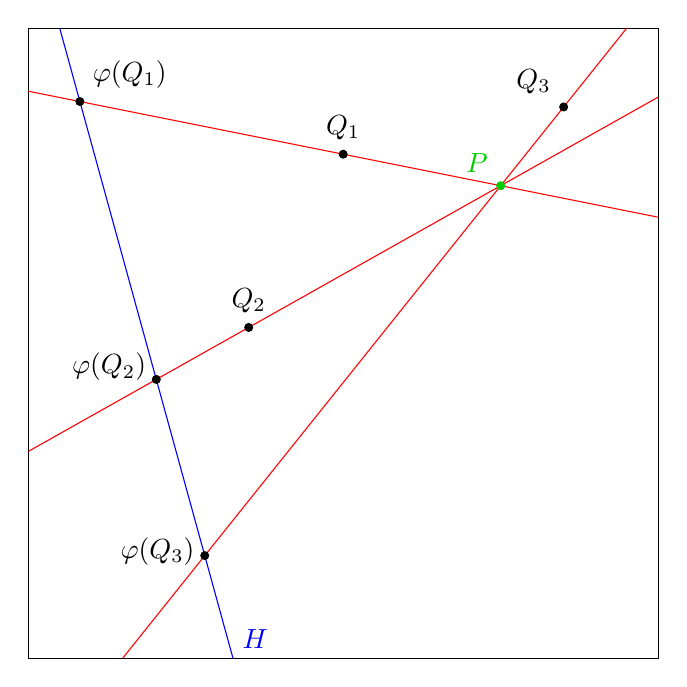
\begin{tikzpicture}[scale=2]
\draw (0,0)--(4,0)--(4,4)--(0,4)--(0,0);
\draw[red] (0,1.3125)--(4,3.5625);
\draw[blue] (0.2,4) -- (1.3,0) node[above right] {$H$};
\draw[red] (0,3.6)--(4,2.8);
\draw[red] (0.6,0)--(3.8,4);

\node[circle, draw, fill, label={[green!80!black]above left:$P$}, inner sep=0.1em, green!80!black] (P) at (3,3) {};
\node[circle, draw, fill, label={above:$Q_1$}, inner sep=0.1em] (Q1) at (2,3.2) {};
\node[circle, draw, fill, label={above right:$\varphi(Q_1)$}, inner sep=0.1em] (pQ1) at (0.32804,3.53439) {};
\node[circle, draw, fill, label={above:$Q_2$}, inner sep=0.1em] (Q2) at (1.4,2.1) {};
\node[circle, draw, fill, label={[shift={(-.6,-.2)}]:$\varphi(Q_2)$}, inner sep=0.1em] (pQ1) at (0.81326,1.76996) {};
\node[circle, draw, fill, label={above left:$Q_3$}, inner sep=0.1em] (Q3) at (3.4,3.5) {};
\node[circle, draw, fill, label={[shift={(-.6,-.3)}]:$\varphi(Q_3)$}, inner sep=0.1em] (pQ1) at (1.12093,0.65115) {};
\end{tikzpicture}
\caption{The projection $\varphi$ away from $P$ in $\P^2$ onto $H \cong \P^1$}
\end{figure}


To honestly check this is a rational map, change coordinates such that $H = \{Z_n = 0\}$ and $P = [0:\ldots:0:1]$. Then the rational map is given by:
\begin{align*}
\P^n &\dashrightarrow \P^n\\
[Z_0\ldots:Z_n] &\mapsto [Z_0:\ldots:Z_{n-1}]
\end{align*}

The \emph{degree d Veronese morphism} is given as follows. Choose a basis for $\mathcal{O}_{\P^n}(d)$, say $F_1, \ldots, F_{\binom{n+d}{d}}$. Then:
\begin{align*}
\mathcal{V}_d:\P^n &\to \P^{\binom{n+d}{d}-1}\\
P &\mapsto [\ldots : F_j(P):\ldots]
\end{align*}
Then the twisted cubic is simply the degree 3 Veronese map of $\P^1$.

Given a rational map $\varphi:X \dashrightarrow Y$ defined by restriction from a rational map $\P^n_K \dashrightarrow \P^m_K$, we define $\Dom \varphi$ to be the  set of all regular points for $\varphi$ on $X$. Then $\varphi$ is said to be \emph{dominant} if $\varphi(\Dom \varphi)$ is Zariski dense.

Let $X$ and $Y$ be irreducible. A rational map $\varphi : X \dashrightarrow Y$ is called \emph{birational} if there exists a rational map $\varphi: Y \dashrightarrow X$ such that $\varphi \circ \psi$ and $\psi \circ \varphi$ are the identity whenever they are defined. We say a projective variety $A$ is birational to another projective variety $B$ whenever there exists some birational map between them, or we might say that $A$ and $B$ are birational.

For example:
\begin{itemize}
\item $A^n$ and $\P^n$ are birational
\item $\V(y^2-x^3)$ is birational to $\A^1$
\item $\V(y^2-x^3+x) \subseteq \A^2_K$ is \textit{not} birational to $\A_K^1$ for $\charr K \neq 2$.
\end{itemize}
\begin{theorem}
Let $X$ and $Y$ be projective varieties. Then $X$ is birational to $Y$ if and only if $K(X) \cong K(Y)$.
\end{theorem}

A \emph{quasi-projective variety} is a Zariski open subset of a projective variety, i.e. $\V(I) \setminus \V(J)$ for two ideals $I, J$. Note that, since $\emptyset$ is a projective variety, every projective variety is also a quasi-projective variety.

\section{Products}
If $X$ and $Y$ are quasi-projective varieties, then $X \times Y$ is also a quasi-projective variety. If $X$ and $Y$ are projective (or irreducible), then $X \times Y$ is also projective (or irreducible), respectively.

This fact relies on the fact that, given $\P^n_K$ and $\P^m_K$, the set $\P^n_K \times \P^m_K$ is naturally a projective variety, and the rest follows from basic topological arguments.

We can approach this from the point of view of creating a Zariski topology on $\P^n_K \times \P^m_K$ using what we already know - a point $P \in \P^n_K \times \P^m_K$ is given by $([a_0:\ldots:a_n],[b_0:\ldots:b_m])$ where we can scale the first and second parts \textit{independently}. We then can consider some appropriate notion of a \emph{bihomogeneous} polynomial in $(n+1)+(m+1)$ variables, obtaining an algebraic structure by using their vanishing loci.

Here however, we will use a slightly different approach:
\subsection{Segre Embedding}
The \emph{Segre embedding} is the map:
\begin{align*}
\sigma_{n,m}:\P^n_K \times \P^m_K &\to \P^{(n+1)(m+1)-1}_K\\
([x_0:\ldots:x_n],[y_0:\ldots:y_m]) &\mapsto [\ldots: x_iy_j:\ldots]
\end{align*}
\begin{claim}
$\sigma_{n,m}$ is injective.
\end{claim}
\begin{proof}
Let $c = [\ldots:C_{ij}:\ldots] \in \Image(\sigma_{n,m})$ and $(a,b) \in \sigma_{n,m}^{-1}(\{c\})$, say $a = [A_0:\ldots:A_n], b = [B_0:\ldots:B_m]$.

We may assume, up to a change of coordinates, that $C_{0,0} = 1$, so $A_0 = B_0 = 1$. This then forces that $B_i = C_{0,i}$ and $A_j = C_{j,0}$, so $a,b$ are unique, so $\sigma_{n,m}$ is injective.
\end{proof}
\begin{claim}
The image of $\sigma_{n,m}$ is closed.
\end{claim}
\begin{proof}
The equations are $\{Z_{ij}Z_{k\ell} - Z_{i\ell}Z_{kj} = 0\}$ for all $i,j,k,\ell$. Checking that $\Image(\sigma_{m,n})$ is equal to the vanishing locus of these equation is a locally affine calculation which is left as an exercise.
\end{proof}
Note that the projection maps
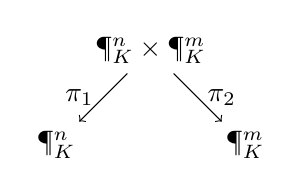
\begin{tikzpicture}
\node (a) at (0,1.2) {$\P_K^n \times \P_K^m$};
\node (b) at (-1.2,0) {$\P_K^n$};
\node (c) at (1.2,0) {$\P_K^m$};
\draw[->] (a) -- node[midway, left] {$\pi_1$} (b);
\draw[->] (a) -- node[midway, right] {$\pi_2$} (c);
\end{tikzpicture}
are both morphisms.

\subsection{The Blow-up}
The \emph{blowup} of $\A^2_K$ at the origin is given as follows:
\begin{align*}
\Bl_{(0,0)}\A^2 = \left\{((x,y),[z:w]) \in \A^2_K \times \P^1_K | xz-yw = 0\right\}
\end{align*}
Since $\A^2 \times \P^1 \to \A^2$ is a morphism, there is an induced morphism:
\begin{align*}
\Bl_{(0,0)}\A^2_K \xrightarrow{\pi} \A^2_K
\end{align*}
If $P \in \A^2_K, P \neq (0,0)$ then $\pi^{-1}(P)$ is exactly one point. In fact, $\Bl_{(0,0)}\A^2 \setminus \pi^{-1}(0,0) \to \A^2_{K}\setminus \{(0,0)\}$ is then invertible, and so $\pi$ is birational map. If instead $P = (0,0)$ then $\pi^{-1}(P) = \P^1_K$.

\begin{figure}
\begin{subfigure}{0.5\textwidth}
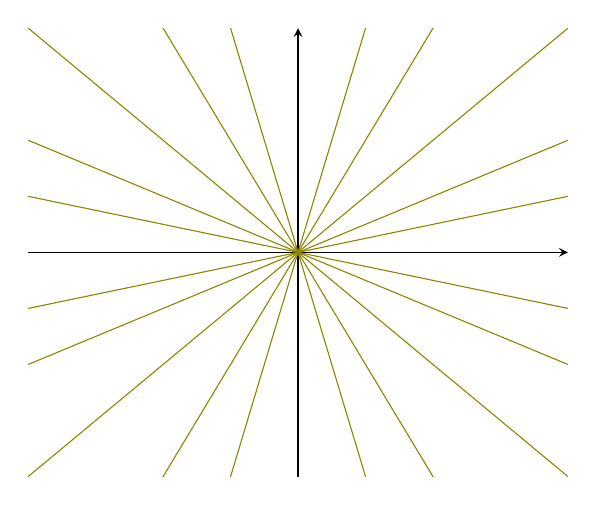
\begin{tikzpicture}
\begin{axis}[axis lines=middle, xmin=-3, xmax=3, ymin=-3, ymax=3, xtick=\empty, ytick=\empty, xticklabels=\empty, yticklabels=\empty]
\addplot[olive, domain=-3:3] (x,x);
\addplot[olive, domain=-3:3] (x,2*x);
\addplot[olive, domain=-3:3] (x,1/2*x);
\addplot[olive, domain=-3:3] (x,4*x);
\addplot[olive, domain=-3:3] (x,1/4*x);
\addplot[olive, domain=-3:3] (x,-1*x);
\addplot[olive, domain=-3:3] (x,-2*x);
\addplot[olive, domain=-3:3] (x,-4*x);
\addplot[olive, domain=-3:3] (x,-1/2*x);
\addplot[olive, domain=-3:3] (x,-1/4*x);
\end{axis}
\end{tikzpicture}
\caption{$\A^2$}
\end{subfigure}
\begin{subfigure}{0.5\textwidth}
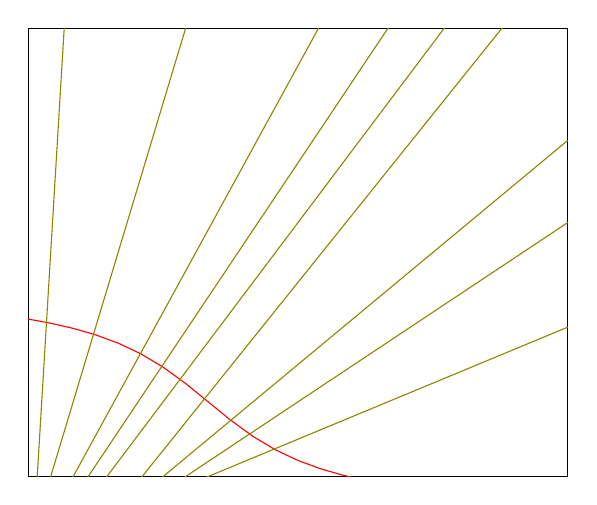
\begin{tikzpicture}
\begin{axis}[xmin=-3, xmax=3, ymin=-3, ymax=3, xtick=\empty, ytick=\empty, xticklabels=\empty, yticklabels=\empty]
\addplot[red, domain=-3:3] (x, {rad(atan(-x-1))-2});
\addplot[olive, domain=-3:3] (x,{1.5*x-0.4});
\addplot[olive, domain=-3:3] (x,{1.6*x+0.4});
\addplot[olive, domain=-3:3] (x,{1.8*x+1.2});
\addplot[olive, domain=-3:3] (x,{2.2*x+2.5});
\addplot[olive, domain=-3:3] (x,{4*x+8});
\addplot[olive, domain=-3:3] (x,{8*x+30});
\addplot[olive, domain=-3:3] (x,{x-1.5});
\addplot[olive, domain=-3:3] (x,{0.8*x-2});
\addplot[olive, domain=-3:3] (x,{0.5*x-2.5});
\addplot[olive, domain=-3:3] (x,{20*x+55});
\end{axis}
\end{tikzpicture}
\caption{$\Bl_{(0,0)}\A^2$}
\end{subfigure}
\end{figure}
We can think of $\P^1$ as separating lines through the origin based on incoming slope. The notion of blowups can be generalised to $\Bl_Z X$ for $Z \subseteq X$ some closed subvariety.

\section{Smoothness, Tangent Spaces, and Dimension}
Given $X \subseteq \P^n_{\C}$ a variety, we want to know when $X$ viewed in Euclidean space is a manifold.
\begin{figure}[H]
\begin{subfigure}{.5\textwidth}
\centering
\begin{tikzpicture}[scale = 1]
\begin{axis}[xticklabels={,,}, yticklabels={,,,}, xtick=\empty, ytick=\empty]
\addplot[blue, ultra thick, domain=-3:3, samples=200] (x, {x^3-3*x});
\end{axis}
\end{tikzpicture}
\caption{$\V(f)$ for $f = y-x^3+3x$}
\end{subfigure}
\begin{subfigure}{.5\textwidth}
\centering
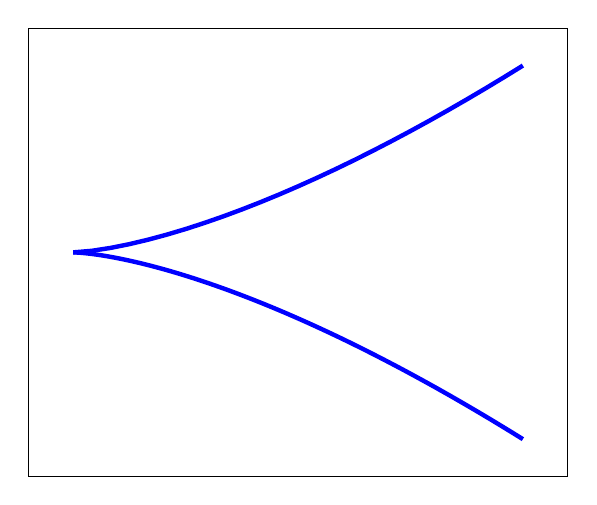
\begin{tikzpicture}[scale = 1]
\begin{axis}[xticklabels={,,}, yticklabels={,,,}, xtick=\empty, ytick=\empty]
\addplot[blue, ultra thick, domain=0:3] (x, {x^(3/2)});
\addplot[blue, ultra thick, domain=0:3, samples=200] (x, {-x^(3/2)});
\end{axis}
\end{tikzpicture}
\caption{$\V(f)$ for $f = y^2-x^3$}
\end{subfigure}
\end{figure}
The curve on the left is smooth, and forms a manifold, whilst the curve on the right has a cusp, so does not form a manifold. We will end up calling it singular.
\subsection{Hypersurfaces}
Let $X = \V(f) \subseteq \A^n_K$. A line in $\A^n_K$ through a point $P = (a_1, \ldots, a_n) \in X$ is given by
\begin{align*}
L = \{ (a_1+b_1t, \ldots, a_n+b_nt)| t \in K\}
\end{align*}
where $(b_1, \ldots, b_n) \in K^n \setminus \{\mathbf{0}\}$. 

We say $L$ is \emph{tangent to X at P} if $g(t) = f(a_1+b_1t, \ldots, a_n+b_nt)$ vanishes to order 2 at $t=0$. More precisely, let
\begin{align*}
f^{lin} \coloneqq \sum_i \frac{\partial f}{\partial z_i}(P)(z_i-a_i)
\end{align*}
be the \emph{linearisation} of $f$ near $P$. Then we can define the \emph{affine tangent space to X at P} by:
\begin{align*}
T_{X,P}^{aff} \coloneqq \V(f^{lin}) \subseteq \A_K^n
\end{align*}
As a sanity check, make sure that this gives the usual tangent line for $y=f(x)$. Note that $T^{aff}_{X,P}$ is centered at the $P$, not at the origin. By shifting it to the origin by translation by $P$, we get the \emph{tangent space to X at P}, given by:
\begin{align*}
T_{X,P}  = \left\{v \in K^n | \sum v_i \frac{\partial f}{\partial z_i}(P) = 0 \;\forall f \in I\right\}
\end{align*}
where $X = \V(I)$. Then $T_{X,P} + P = T_{X,P}^{aff}$.

For example, in the case $X = \V(y^2-x^3)$, we calculate $f^{lin}$ at $(0,0)$ to be $0$, and so $T_{X, (0,0)}^{aff}$ is $\A^2_K$.

\subsection{Digression On Cubics}
Let $f_2 \in \mathcal{O}_{\P^2}(3)$ such that $\V(f_2)$ is smooth. Then $\V(f^2)$ is an \emph{elliptic curve}. In particular, $K(E)$ is not isomorphic to $K(z)$. We say that $X$ is \emph{rational} if $X$ is birational to $\P^r$ for some $r$.

Let $f_3 \in \mathcal{O}_{\P^3}(3)$. We call $\V(f_3)$ a \emph{cubic surface}. We'll take $f_3 = z_0^2z_1 + z_1^2z_2 + z_2^2z_3+z_3^2z_0$, and let $S = \V(f_3)$. Consider the rational map $\varphi: S \dashrightarrow \P^2$, taking $[z_0:\ldots:z_3]\mapsto [z_0z_3:z_1z_2:z_2z_3]$. We can also take some map $\psi:\P^2 \dashrightarrow S$ such that $\varphi\circ\psi$ and $\psi \circ\varphi$ are the identity map, and so $K(S) = K(z_1,z_2)$, and $S$ is smooth. This holds for any smooth cubic surface in $\P^3_K$, and they are all rational.

If $f_4 \in \mathcal{O}_{\P^4}(3)$, then $\V(f_4) = X$ is sometimes called a \emph{cubic threefold} - it was a landmark result of the late 20\th century to prove that $X$ is not rational.

If $f_5 \in \mathcal{O}_{\P^5}(3)$. and $Y=\V(f_5)$ is a smooth \emph{cubic fourfold}, then the rationality of $Y$ is an open question.

\subsection{Dimension and Smoothness}
Let $X$ be an irreducible variety. Then we define the \emph{dimension} of $X$ as:
\begin{align*}
\dim X = \min_{p \in X} \{\dim T_{X,p}\}
\end{align*}
If $X$ is reducible, the we can write it uniquely as a union of irreducible varieties $X_1 \cup \ldots \cup X_n$, and let $\dim X = \max_{i}\dim X_i$. If all $X_i$ have the same dimension, then $X$ is \emph{pure}.

A point $p \in X$ is said to be \emph{smooth} if $\dim_K X = \dim_K T_{X, p}$, and a non-smooth point is said to be \emph{singular}.

\begin{proposition}
Let $X$ be a variety. Then the set of singular points is a closed proper subvariety.
\end{proposition}
\begin{proof}
It suffices to treat the case where $X$ is affine so $X  = \V(I)$ for $I = \angle{f_1, f_2, \ldots, f_n} \subseteq K[\mathbf{x_i}]$.

Treating $\left(\frac{\partial f_j}{\partial z_i}(p)\right)$ as a matrix, we then have from the definition $\dim_K T_{X,p} = n-\rank \left(\frac{\partial f_j}{\partial z_i}(p)\right)$. The locus where this rank is $\leq n-r$ for any $r \in \N$ is the closed subvariety given by the vanishing of the $(n-r)\times (n-r)$ minors.
\end{proof}
Morally what this tells us, since open subsets of varieties are dense, is that most points on an algebraic variety are smooth points.

\begin{proposition}
If $X$ and $Y$ are irreducible and birational then $\dim X = \dim Y$.
\end{proposition}

Let $\phi : X \dashrightarrow Y$ be a rational map regular at $p \in X$, where $X \subseteq \A_K^n, Y \subseteq \A_K^m$. Then we can write $\phi = (f_1, \ldots, f_m)$, where $f_j \in K(z_1, \ldots, z_n)$ is regular at $p$. We can then define $d\phi_p : T_{X,p} \to T_{Y, \phi(p)}$, the \emph{differential of $\phi$ at p}, defined by:
\begin{align*}
d\phi_p(\mathbf{v}) = \left(\sum_{i=1}^n v_i \frac{\partial f_j}{\partial z_i}(p)\right)_j
\end{align*}
It follows from the chain rule that $d\phi_p(\mathbf{v})$ does indeed lie in $T_{Y, \phi(p)}$ - checking this is left as an exercise.

If $X \dashrightarrow_\phi Y \dashrightarrow_\psi Z$, and $p \in \dom(\phi)$, $\phi(p) \in \dom(\psi)$, then $d\psi_{\phi(p)}\circ d\phi_p = d(\psi \circ \phi)_p$.

Proposition \textbf{6.2} follows immediately from this.

We might ask the following question: if $X$ is a variety, is $X$ isomorphic to a \emph{hypersurface}? The answer to this question is no - consider $X = \V(xy,yz,zx)$, a union of the coordinate axes in $\A^3$. We might think this is isomorphic (it is certainly \textit{homeomorphic}) to a \emph{planar triple point}, e.g. $\A^2 \supseteq Y = \V(xy(x-y))$. Then $X \ncong Y$ because the dimension $T_{X,(0,0,0)}$ is 3, and $Y$ can have no such point.

\begin{theorem}
Given any irreducible variety $X$ there exists a hypersurface $Y$ such that $X$ is birational to $Y$, i.e. $K(X) = K(Y)$.
\end{theorem}
The proof of this will come later, but first we'll have a short digression on field theory.

Let $L$ be a finitely generated field extension of $K$. The field $L$ is called a \emph{purely transcendental extension} of $K$ if there exist elements $x_1, \ldots, x_n$ algebraically independent\footnote{i.e. with no polynomial equation in $x_i, i \neq j$ with $x_j$ a root.} over $K$ such that $L = K(x_1, \ldots, x_n)$.

\begin{proposition}
Let $L/K$ be a finitely generated field extension. Then there exists a subfield $K \subseteq M \subseteq L$ purely transcendental over $K$ such that $L/M$ is algebraic and separable. Moreover, $L = M(y)$ for some $y \in L$.
\end{proposition}
\begin{proof}[Proof (Characteristic 0)]
Since $L$ is finitely generated, we know that $L = K(x_1, \ldots, x_m)$. There is a maximal algebraically independent subset of $\{x_i\}$. Re-order this set such that $\{x_1,\ldots, x_n\}$ form this subset. Then take $M = K(x_1, \ldots, x_n)$, which is purely transcendental. Then by finite generation $L/M$ is finite and algebraic, and in characteristic 0 separability is automatic. For the final statement, apply the theorem of the primitive element.
\end{proof}
The integer $n$ will turn out to be unique and equal to $\dim X$ where $X$ is a variety with $K(X) = L$.
\begin{proposition}
Let $L = K(x_1, \ldots, x_n)$ be pure transcendental, and $x_{n+1}$ is algebraic. Then the ideal $I = \{g \in K[z_1, \ldots, z_{n+1}] : g(\mathbf{x}) = 0\}$ is principal, i.e. $I = (f)$. Moreover, if $f$ contains the variable $z_i$, then the set $\{x_1, \ldots, x_{i-1}, x_{i+1}, \ldots, x_{n+1}\}$ is algebraically independent.
\end{proposition}
\begin{proof}
Since $\{x_i\}$ are algebraically independent, the subring $L \supseteq R = K[x_1, \ldots, x_n]$ is isomorphic to the polynomial ring in $n$ variables, and in particular is a UFD.

Then let $h \in L[t]$ be the minimal irreducible polynomial for $x_{n+1}$. Let $b$ be the LCM of the denominators of its coefficients. So then if we take $f = b\cdot h$, where $f \in K[x_1, \ldots, x_n, t]$. Since $h$ is irreducible, the Gauss lemma implies that $f$ is irreducible in $R$.

Let $g \in K[z_1, \ldots, z_{n+1}]$ be an element of $I$. In $K[t]$, $g$ is a multiple of $h$. Again by the Gauss lemma, if $h$ divides $g$ then $f$ divides $g$, and so $I$ is principal and generated by $f$.

For the last part, assume $\{x_1, \ldots, x_{i-1}, x_{i+1}, \ldots, x_{n+1}\}$ was algebraically dependent. Then there exists $g \in I$ not containing $z_i$ such that $g(x_1, \ldots, x_{n+1}) = 0$. But $f$ divides $g$, which is a contradiction.
\end{proof}
\begin{corollary}
If $X$ is an irreducible variety and $K(X)$ is its function field, then:
\begin{align*}
\dim X = \tr \deg_K K(X)
\end{align*}
\end{corollary}
\begin{proof}
Exercise - reduce the the case where $X = \V(f)$ and apply the second part of the previous proposition.
\end{proof}
\begin{proof}[Proof of 6.3]
Given $X$ irreducible, apply the \textbf{6.5} to $K(X)$. So $K(X) \equiv \text{FractionField}(K[z_1, \ldots, z_n]/(f))$
\end{proof}
\begin{theorem}[Affine Nullstellensatz I]
Every maximal ideal in $K[z_1, \ldots, z_n]$ is of the form $m  = (z_1a_1, \ldots, z_na_n)$ for $a_i \in K$. If $I\subsetneq K[\mathbf{z}_i]$ is a non-unit ideal, then $\V(I) \neq \emptyset$.
\end{theorem}
\begin{proof}[Proof in uncountable case]
For the first part, clearly every ideal of that form is maximal. Conversely, let $m \subseteq K[\mathbf{z}_i]$. Consider $L = K[\mathbf{z}_i]/m$, which is a field, and let $a_i = z_i + m$. If $L = K$, then $a_i \in K$ as required. Otherwise, $L/K$ must be transcendental.

Take $t \in L\setminus K$. Then $K \subseteq K(t) \subseteq L$, and $t$ is transcendental. now, let $U_m = \angle{a_1^{m_1}\ldots a_n^{m_n}}$ where $\sum m_i = m$. These are all finite dimensional over $K$, but $\bigcup_m U_m = K$. Observe for each $c \in K$, the elements $\frac{1}{t-c}$ are linearly independent. But there are uncountably many of them. Only finitely many lie in each $U_m$, so we get a contradiction.
\end{proof}

\section{Curves}
An \emph{algebraic curve} is an algebraic variety of dimension 1. 
\begin{proposition}
If $X$ is an irreducible curve and $W \subseteq X$ is a proper closed subvariety, then $w$ is finite.
\end{proposition}
\begin{proof}
We've already proven this for plane curves. We can assume $X$ is affine and let $I(X)$ be the associated ideal, and that $W$ is irreducible. By the Nullstellensatz, we know that $I(X) \subsetneq I(W)$, and let $\varphi : W \injection X$ be the inclusion map - this induces a homomorphism of coordinate rings given by restriction $\varphi^{\ast}: K[X] \to K[W]$.

If $W$ is not a point, then $K[W] \neq K$, so take $t \in K[W] \setminus K$. The element $t$ is transcendental over $K$. Then take $0 \neq x \in K[x]$ with $\varphi^{\ast}(x) = 0$ and $y \in K[X]$ with $\varphi^{\ast}(y) = t$. Note that $x$ and $y$ are algebraically independent, but $\dim X = 1\implies \tr \deg K(X) = 1$ so we get a contradiction.
\end{proof}
\subsection{Basic Structure on Curves}
Let $X$ be an irreducible curve. Given $p \in X$, the \emph{local ring of X at p} is defined to be $\mathcal{O}_{X,p} = \mathcal{O}_p = \{\frac{f}{g} : f,g \in K[X], g(p) \neq 0\}$ - the functions defined on some open set containing $p$.

Then $\mathcal{O}_{X,p} \supseteq m_p = \{F \in \mathcal{O}_{X,p} : F(p) = 0\}$. It is an easy exercise to show that $m_p$ is an ideal, and almost as easy to show that it is maximal. Moreover, $\mathcal{O}_{X,p} \setminus \mathcal{O}_{X,p}^{\ast}$, the set of non-units in $\mathcal{O}_{X,p}$, is precisely $m_p$, so $m_p$ is the unique maximal ideal in $\mathcal{O}_{X,p}$.

This definition of a local ring is similar to one from commutative algebra: a \emph{local ring} is a commutative ring that is not a field with a unique maximal ideal.

For example, if $X$ is an irreducible curve, $\mathcal{O}_{X,p}$ is a local ring. Other examples of local rings include $\C\llbracket t\rrbracket$, the formal power series in $t$, with unique maximal ideal generated by $t$. 

\begin{theorem}
If $X$ is an irreducible curve and $p \in X$ is a smooth point, then the ideal $m_p \trianglelefteq \mathcal{O}_{X,p}$ is principal.
\end{theorem}
We will refer to a generator of $m_p$ as a \emph{local parameter/coordinate} at $p$.
\begin{proof}
Assume $p \in X_0 \subseteq \A_K^n$ is an affine patch of $X$ at $p$. After a change of coordinates, we can assume that $p$ is the origin. We can write $K[X_0] = \frac{K[z_1, \ldots, z_n]}{I(X_0)} = K[x_1, \ldots, x_n]$ as an algebra \underline{\textsc{not}} as a polynomial ring - the $x_i$s can have relations. They are just the images of the $z_i$s under the quotient map.

Then $\mathcal{O}_{X,p} = \mathcal{O}_{X_0,p} = \{\frac{f}{g} : f,g \in K[X_0], g \notin (x_1, \ldots, x_n)\}$. So then $m_p = \{\frac{f}{g} : f,g \in K[X_0], f \in (x_1, \ldots, x_n), g \notin (x_1, \ldots , x_n)\} = x_1\mathcal{O}_{X,p} + \ldots + x_n\mathcal{O}_{X,p}$.

We change coordinates, so that $T_{X,p}^{aff} = T_{X,p} = \{z_2 = z_3 = \ldots = z_n = 0\}$. Since the $z_i$ linearise equations for $X_0$, there exist functions $f_2, \ldots, f_n \in I(X_0)$ such that $f_i = z_i - h_i$ where $h_i$ has no terms of degree $\leq 1$. In $\mathcal{O}_{X,p}$ we have $x_i = h_i(x_1, \ldots, x_n) \in (x_1^2, x_1x_2, \ldots, x_n^2) = m_p^2$.

Note that this implies that the image of $x_1$ inside $m_p/{m_p^2}$ is a generator as a $K$-vector space, $K[X_0]/m = \mathcal{O}_{X,p}/{m_p}$.

In turn, by applying Nakayama's Lemma, we can conclude that $x_1$ generates $m_p$.
\end{proof}
\begin{lemma}[Nakayama's Lemma]
Let $R$ be a local ring with maximal ideal $m$, and let $M$ be a finitely generated $R$-module. If $mM = M$ then $M = 0$.
\end{lemma}
\begin{proof}
\google
\end{proof}
\begin{corollary}
If $(R,m)$ are as above, and if $t_1, \ldots, t_r \in m$ generate $m/m^2$, as an $R/{m}$-vector space, then they generate $m$.
\end{corollary}
This is the corollary we need to finish off the proof.
\begin{proof}
Let $n = \angle{t_1, \ldots, t_n} \subseteq m$. If the images of $\{t_i\}$ generate $m/{m^2}$, then $n+m^2 = m+m^2 \implies n+m^2/n = m+m^2/n \implies m(m/n) = (m/n)$. So by Nakayama, $m/n = 0$, and $m = n$.
\end{proof}

\begin{corollary}
If $X$ is an irreducible curve and $p \in X$ be a smooth point, then the maximal ideal $m_p \subseteq \mathcal{O}_{X,p}$ of functions vanishing at $p$ is principal, and $\mathcal{O}_{X,p}$ is a discrete valuation ring, i.e. there exists $\ord_p : K(X)^\ast \to \Z$ such that:
\begin{align*}
\mathcal{O}_{X,p} &= \{f \in K(X)^\ast |\ord_p(f) \geq 0\} \cup \{0\}\\
m_p &= \{f \in \mathcal{O}_{x,p} : \ord_p(f) > 0\}\cup\{0\}
\end{align*}
\end{corollary}
\begin{proof}
We know $m_p = (\pi_p)$ as $m_p$ is principal by \textbf{7.2}, and so $m_p^n = (\pi_p^n)$. We will examine $J = \bigcap_n m_p^n$. Observe that $m_p J = J$, so $J = 0$ by Nakayama's lemma.

Then for $f \in \mathcal{O}_{X,p}$, define $\ord_p(f)$ to be the largest $n \in \Z_{\geq 0}$ such that $f \in m_p^n$. If $f \in K(X)^\ast\setminus \mathcal{O}_{X,p}$, then $f^{-1} \in \mathcal{O}_{X,p}$. In this case, we define $\ord_p(f) = -\ord_p(f^{-1}) \in \Z_{\leq 0}$.
\end{proof}
We will also use $v_p(x) = \ord_p(x)$ as an alternative notation. By convention, we wil say that $v_p(0) = +\infty$, so that $v_p:K(X)^{\ast} \to \Z\cup\{\infty\}$.

\begin{corollary}
If $X$ is a smooth projective curve and $X \dashrightarrow_\varphi \P^m$ is a rational map then $\varphi$ is a morphism.
\end{corollary}
\begin{proof}
Let $\varphi = (\varphi_0, \ldots, \varphi_m)$ and $p \in X$ as above. Pick a local parameter $\pi_p$ at $p$, and calculate $\min_i\{v_p(\varphi_i)\} = n$, say. Then replace $(\varphi_0, \ldots, \varphi_m)$ with $(\pi_p^{-n}\varphi_0, \ldots, \pi_p^{-n}\varphi_m)$ to get an equivalent rational map, but this time regular at $p$.
\end{proof}

\begin{corollary}
Any birational map of smooth projective curves
\begin{align*}
\varphi: X_1 \dashrightarrow X_2
\end{align*}
is an isomorphism. A smooth projective curve is uniquely determined by the field of functions. 
\end{corollary}
\begin{theorem}
The image of a projective variety under a morphism is closed.
\end{theorem}
\begin{proof}
\google
\end{proof}
\begin{corollary}
Any morphism of projective irreducible curves is either surjective or constant.
\end{corollary}
\begin{proof}
Given $\varphi:X_1\to X_2$, since $\varphi(X_1)$ is closed and connected, then $\varphi(X_1) = X_2$ or $\varphi(X_1) = \bullet$.
\end{proof}
\begin{proposition}
Let $\varphi:X_1 \to X_2$ be a non-constant morphism of algebraic curves. Then:
\begin{itemize}
\item $\varphi$ is a finite map, i.e. $|\varphi^{-1}(p)|<\infty$ for all $p \in X_2$
\item We have a pullback $\varphi^\ast:K(X_2)\injection K(X_1)$ exhibiting $K(X_1)$ as a finite algebraic extension of $K(X_2)$.
\end{itemize}
\end{proposition}
\begin{proof}
The first statement is clear since $\varphi^{-1}(p)$ is closed for all $p \in X_2$. For the second part, observe that $\varphi(X_1)$ is infinite since $k = \bar{k}$ so $\varphi(X_1)$ is dense, so $\varphi^\ast$ makes sense. Now $K(X_2)$ lives inside $K(X_1)$ which is transcendental over $K$ but algebraic over $K(t)$, so the extension $[K(X_1):K(X_2)]$ is finite.
\end{proof}
The number of preimages of $p \in X_2$ is finite, but can depend on the choice of $p$. For example, if we take $\P^1_{\C} \to \P^1_\C$ by squaring. Then $\varphi^{-1}(0) = 0, \varphi^{-1}(\infty), \varphi^{-1}(a) = \pm \sqrt{a}$.

Given $\varphi:X_1\ to X_2$ a morphism of irreducible curves, the \emph{degree of $\varphi$}, $\deg \varphi = \deg[K(X_1):K(X_2)]$. When $\varphi^\ast$ is separable, it is a fact that $\deg \varphi$ is equal to the maximum number of preimages of points in $X_2$. Store this fact as true without asking for proof, or just \google it.

What about the non-generic points in $X_2$ and their preimages?

Given $\varphi: X_1 \to X_2$ as before and $p \in X_1$, define the \emph{ramification index} of $\varphi$ at $p$ to be $\ord_p (\varphi^{\ast} \pi_q )$ where $\pi_q$ is a local parameter for $X_2$ near $\varphi(p) = q$.

\begin{theorem}
Let $\varphi:X_1 \to X_2$ be a morphism of projective irreducible curves.
\begin{enumerate}
\item If $\varphi$ is non-constant, then $\varphi$ is surjective.
\item If $X_1$ and $X_2$ are smooth, then for any $q \in X_2$, $\deg \varphi = \sum_{p \in \varphi^{-1}(q)} e_p$ where $e_p$ is the ramification index at $p$.
\item If $\charr(K) = 0$ or if $\varphi^{\ast}$ is separable, then $e_p = 1$ generically, i.e. outside a finite set.
\end{enumerate}
\end{theorem}
\begin{proposition}
Let $X$ be a smooth projective curve and $f \in K(X)$ is regular for all points $p \in X$. Then $f \in K$.
\end{proposition}
\begin{proof}
Examine $\varphi= 1\cdot f : X \to \P^1$. The image must include $\infty$ if $\varphi$ is non-constant, but this contradicts regularity of $f$.
\end{proof}

\subsection{Brill-Noether Problem}
Let $X$ be a smooth projective irreducible curve. For what integers $r, d \geq 0$ does $X$ admit a morphism (embedding):
\begin{align*}
X \xrightarrow{\varphi} \P_K^r
\end{align*}
where $\varphi$ has degree $d$? ($\varphi(x)$ should not be contained in a hyperplane). (We say the \emph{degree} of $\varphi$ is the number of preimages of a generically chosen hyperplane in $\P^r$).

We won't answer this question because it is too hard, but we will try to make some progress in this direction. We will need the Riemann-Roch theorem, Riemann-Hurwitz theorem, and the ideas of genus and canonical divisor.

Let $X$ be a curve and $\varphi:X \to \P^r_K$ be a morphism. The map $\varphi$ is given by rational functions $(\varphi_0, \ldots, \varphi_r)$. If we consider the open set $\P^r_K\setminus \{z_r = 0\}$, we can divide by $\varphi_r$ to get $\left\{\frac{\varphi_i}{\varphi_r}\right\}_{i=0}^{r-1}$ rational function on an open set of $X$.

In other words, given $\varphi:X \to \P^r_K$ we get $r$ rational functions, say $f_1, \ldots, f_r \in K(X)$ which are undefined on precisely the same points: where $\varphi_r = 0$. In fact we can say more - they are also undefined in the same way in the sense of orders of poles from complex analysis: given $f \in K(X)$ and $p \in X$, we say that $f$ has a \emph{pole} at $p$ if $\ord_p(f) < 0$, and that the order of this pole is $-\ord_p(f)$.

A \emph{divisor} $D$ on a curve $X$ is an element of the group $\Div(X) = \bigoplus_{p \in X}\Z p$ - all finite $\Z$-linear combinations of points. The \emph{degree} of a divisor $D = \sum a_i p_i$ is given by $\deg D = \sum a_i$. As a point of notation, $\Div^d(X) = \{D \in \Div(X) : \deg D = d\}$.

A rational function $f \in K(X)^{\ast}$ gives rise to a divisor as follows:
\begin{align*}
\div(f) = \sum_{p\in X} \ord_p(f) \cdot p
\end{align*}
\begin{lemma}
For $f \in K(X)^{\ast}$, $\div(f) \in \Div(X)$, i.e. $\ord_p(f) = 0$ for all but finitely many $p \in X$. In fact, $\deg(\div(f)) = 0$.
\end{lemma}
\begin{proof}
Given $f$, take $\varphi: X \to \P^1; x\mapsto [1:f(x)]$. We need to calculate the zeroes and poles of $f$, which correspond to the points of $X$ mapping to $0$ and $\infty$ respectively. Take a local parameter $t$ around $0$ and $\frac1t$ around $\infty$. Then applying the results from the basic structure on curvs:
\begin{align*}
\deg(\varphi) = \sum_{p\in X, p \mapsto 0} e_p = \sum_{p \in X, p \mapsto \infty} e_p
\end{align*}
where in each case the $e_p$s give the orders of zeros and poles.  In particular, the weighted numbers of zeroes and poles are equal.
\end{proof}
The image of the homomorphism $\div$ is contained in $\Div^0(X)$, and is called the \emph{set of principal divisors}.
\begin{proposition}
Every degree 0 divisor on $\P^1$ is principal.
\end{proposition}
\begin{proof}
Exercise.
\end{proof}
The \emph{Jacobian group} of $X$ is $\Div^0(X)/\{\div(f):f\in K(X)^{\ast}\}$, and the \emph{Picard group} of $X$ is $\Div(X)/\{\div(f): f \in K(X)^{\ast}\}$.

As a fun fact, over $\C$, $\Jac(X)$ is a projective variety, and is homeomorphic to $(S^1)^g$ for some $g \in \N$.

\subsection{Hyperplane Sections}
Given $X \subseteq \P_K^r$, the coordinate functions on $\P_K^r \setminus \{z_r = 0\}\cong \A^r_K$ give rational function on $X$ which are morphisms away from $X \cap \{Z_r = 0\}$. Let $L \in \mathcal{O}_{\P^r}(1)$ and $H = \V(L)$ and $X \nsubseteq H$. Then define $\div(L) = \sum_{p\in X}n_p p$,where $n_p = v_p(L/z_i)$ for any coordinate $z_i(p) \neq 0$ - this doesn't depend on $i$. Then $n_p$ is nonzero only for $p \in Z \cap H$. Note that these are not principal because $\deg L$ is $\geq$ than the number of intersection points of $X$ and $H$.

Keep in mind that $\overline{\V(y-x^2)}$ in $\P^2$, then $\div(X)$ is $2\cdot(0,0)$.

Given $D, E \in \Div^d(X)$, we say that $D \thicksim E$ (linear equivalence) if $D-E = \div f$. 

\begin{proposition}
Given $X \subseteq \P_K^r$ and $L_1, L_2 \in \mathcal{O}_{\P^r}(1)$ such that $\V(L_i) \nsupseteq X$, then $\div(L_1) \thicksim \div(L_2)$.
\end{proposition}
\begin{proof}
$\div(L_1) - \div(L_2) = \div(L_1/L_2)$.
\end{proof}

If $X$ is a projective curve it can be exhibited as $\V(I) \subseteq \P^N$ for different choices of $I, N$. Is there a canonical way of doing so?

Last time, we saw that, given $X \subseteq \P^r$ a curve and $L \in \mathcal{O}_{\P^r}(1)$ and $H = \V(L)$, we obtained a divisor on $X$ whose support lies on $H \cap X$, defined by $\div(L) = \sum n_p p$ where $n_p = \ord_p(L/z_i)$ for some $z_i(p) \neq 0$.

If $H$ is chosen generically then $\div(L) = \sum_{p\in X} [p]$. For divisors $D_1, D_2$ given by $D_i = \div(L_i)$, where $L_1, L_2 \in \mathcal{O}_{\P^r}(1)$, the principal divisor. $\div(L_1/L_2) = D_1-D2 \implies D_1 \thicksim D_2$.

There's no reason to restrict $H$ to be a hyperplane - any hypersurface will do. Analogously, given $F \in \mathcal{O}_{\P^r}(d)$ with $\V(F) \nsupseteq X$, we can define $\div(F)$ on $X$ by taking $n_p = \ord_p(F/z_i^d)$ for $z_i(p) \neq 0$.

\begin{theorem}[Bezout's Theorem]
Given $X \subseteq \P^2$ and $Y = \V(F)$, $F \in \mathcal{O}_{\P^2}(d)$. If $\deg(X) = c$, then $\#(X\cap Y) \leq cd$, and we have equality if we count with multiplicity.
\end{theorem}
\begin{proof}
Take $F = \prod_{i=1}^d L_i$, of generically chosen linear forms, and then reduce to the case already proved.
\end{proof}
A divisor $D \in \Div(X)$ is \emph{effective} if $D = \sum n_p[p]$ with $n_p \geq 0$.

Let $D$ be a divisor. We want to consider rational functions on $X$ with poles bounded by $D$. We define:
\begin{align*}
L(D) = \{0\} \cup \{f \in K(X)^{\ast} : \div(f) + D\text{ is effective}\}
\end{align*}
It is easy to see that this is a vector space over $K$. It is harder to see that if $D \thicksim E$ then there is an isomorphism $L(D) \xrightarrow{\cong}L(E)$, and it is a non-examinable fact that $L(D)$ is always finite dimensional.

If $D \thicksim E$ then $D-E = \div(g)$ for $g \in K(X)^{\ast}$. Now observe that multiplication by $g$ gives $L(D) \xrightarrow{\times g} L(E)$.

Given $L(D)$, if we choose a basis $F_1, \ldots, F_s$, we obtain a morphism:
\begin{align*}
X &\to \P^s\\
p &\mapsto [1:F_1(p):\ldots:F_s(p)]
\end{align*}
\begin{proposition}
Given a divisor $D$, let $\ell(D) = \dim_K L(D)$.
\begin{enumerate}
\item If $\deg D < 0$, then $\ell(D) = 0$.
\item For any $p \in X$, $\ell(D) \leq \ell(D-p)+1$.
\item If $\deg D \geq 0$, $\ell(D) \leq d+1$.
\end{enumerate}
\end{proposition}
\begin{proof}
\item
\begin{enumerate}
\item Suppose $f \in L(D)$ is nonzero. Then $E = \div(f) + D \geq 0$, so is effective. But $E$ has the same degree as $D$ since $\deg(\div(f)) = 0$ \contr.
\item Consider the following map. If $p \in X$ and $n = n_p$, writing $\sum n_p[p] = D$, pick a local parameter at $p$ and consider:
\begin{align*}
L(D) &\to K\\
f &\mapsto \pi_p^n f(p)
\end{align*}
$L(D-p)$ is the kernel of this map.
\item Apply 2. repeatedly.
\end{enumerate}
\end{proof}
The residue theorem from complex analysis says that, given a meromorphic function on $\P^1$, $\sum_{p \in \P^1} Res(f,p) = 0$. There is a similar statement for Riemann surfaces.

\subsection{Differentials}
Let $L/K$ be an extension. The space of \emph{Kahler differentials} is the quotient $M/N$ where $M = \text{vector space over $K$ generated by symbols } \delta x, x \in L$, and $N$ is the vector space of relations given by $\delta(x+y)=\delta x+\delta y$, $\delta(xy) = x\delta y+y\delta x$, $\delta a =0$ for $a \in K$. 

The image of $\delta x$ in $M/N$ is denoted $dx$. We define $\Omega_{L/K} = M/N$. There is a canonical map $K \to \Omega_{L/K}$, $f \mapsto df$.

We will now develop a meaningful way to take $\omega \in \Omega_{L/K}$ for $L = K(X)$, and produce a canonical divisor class $\div(\omega) \in \Pic(X)$.

A \emph{K-linear derivation} is an $L$-vector space $U$ and a map $D: L \to U$ satisfying the product rule $D(xy) = xD(y) + yD(x)$. For any $K$-derivation $D$ there exists a unique factorization making
\begin{center}
\begin{tikzpicture}
\node (o) at (0,0) {$\Omega_L$};
\node (u) at (3,0) {$U$};
\node (k) at (1.5,-1.5) {$L$};
\draw[->] (o) -- node[above] {$\lambda$} (u);
\draw[->] (k) -- (u);
\draw[->] (k) -- (o);
\end{tikzpicture}
\end{center}
commute. Moreover, every derivation to a vector space $U$ is given by such a $\lambda$.

\begin{lemma}
If $f = g/h$ for $g, h \in K[z_1, \ldots, z_n]$ such that $y = f(x_1, \ldots, x_n) \in L$ (and so $x_i \in L$), then:
\begin{align*}
dy = \sum_{i=1}^w \frac{\partial f}{\partial z_i}(z_1, \ldots, x_n) dx_i
\end{align*}
If $L = K(x_, \ldots, x_n)$, then $\Omega_L$ is spanned by $dx_1, \ldots, dx_n$
\end{lemma}
\begin{proof}
The first part follows by calculus - this is precisely how we constructed $\Omega_L$, and the second follows from the first.
\end{proof}
\begin{lemma}
Let $K(x)$ be purely transcendental and $L/K(x)$ be a finite and separable extension. Then $\Omega_L$ is spanned by $dx$.
\end{lemma}
\begin{proof}
If $L = K(x)$ then $\dim_L \Omega_L \leq 1$. To show that $\Omega_L$ is nonzero, it suffices to exhibit a nonzero derivation. Take $\frac{d}{dx}:K(x) \to K(x)$. If $L \neq K(x)$ then take $L = K(x, \alpha)$ where $\alpha$ is algebraic over $K(x)$ by the primitive element theorem. Let $L_0 = K(x)$, and $h(y) \in L_0[y]$ be the minimal polynomial of $d$. Then:
\begin{align*}
0 = d(h(\alpha)) = D_x h(\alpha)dx + h'(\alpha) d\alpha
\end{align*}
So $d\alpha$ lies in the span of $dx$, and so $dx$ spans $\Omega_L$. To show that $\Omega_L$ is nonzero, we'll exhibit a derivation on $L = L_0(\alpha) = L_0[y]/h(y)$.

We then define $D: L_0[y] \to L$ by, if $f \in L_0$, then $D(f) = D_x(f)$, and otherwise $D(y) = \frac{-D_x(h(\alpha))}{h'(\alpha)}, D(y^n) = n\alpha^{n-1}D(y)$. We can check this vanishes on $(h)$, and so gives a derivation on $K$, and its restriction to $L_0$ is the derivation $\frac{d}{dx}$, so is nonzero.
\end{proof}
Given a point $p \in X$, we define the \emph{meromorphic differentials on $X$ that are regular at p}, $\Omega_{X,p} = \{\omega \in \Omega_L : \exists f_i, g_i \in \mathcal{O}_{X,p}: \omega = \sum f_i dg_i\}$.
\begin{proposition}
The $\mathcal{O}_{X,p}$-module $\Omega_{X,p}$ is freely generated by $d\pi_p$, where $\pi_p$ is any local parameter at $p$.
\end{proposition}
\begin{proof}[Sketch proof]
Firstly we show that $\Omega_{X,p}$ is finitely generated, which is done by choosing an affine chart, and then we apply Nakayama's lemma.
\end{proof}
Given this, let $\omega \in \Omega_L$, then we can define a divisor:
\begin{align*}
\div(\omega) = \sum_{p \in X} n_p[p], n_p \coloneqq \ord_p(f), \omega = f\cdot d\pi_p
\end{align*}
\hspace{1em}\example Let $X = \P_K^1$, with coordinate $t$, and take $\omega = dt$. A local parameter at any point $p \neq \infty$ is given by $t$. Thus $v_p(\omega) = 0$ for all $p \neq \infty$, as $1$ vanishes to order 0 everywhere. Near $\infty$, the local parameter is $1/t$, so $dt = t^{-2}d(1/t)$, so $\div(\omega) = -2[\infty]$.

Let $\omega \in \Omega_K$. Then the class of $[\div(\omega)] \in \Pic(X)$ is called the \emph{canonical divisor class}, and is denoted $K_X$. The \emph{genus} of an algebraic curve $X$ is defined to be:
\begin{align*}
g(X) = \dim_K L(K_X)
\end{align*}

If $X$ is a curve over $\C$, we can consider the associated Euclidean topological space over $\R$. If $g(X) = g$, then $X$ is determined up to homeomorphism to be a genus $g$ surface in the topological sense. It is useful to think of $g(X)$ as begin related to the curvature of $X$, where $g=0$ means positive curvature, $g=1$ means no curvature, and $g\geq 2$ means negatively curved.

So now our goal is to compute $\ell(D)$ for some divisor $D$ based on $d = \deg D$ and $g = g(X)$.

\begin{theorem}[Riemann]
$\ell(D) \geq d-g+1$, where $\ell(D) = \dim_K L(D)$.
\end{theorem}
Note that if $X = \P^1$, then $\ell(D) = d+1$, as $D \equiv d[\infty]$ by example sheet 3, so $L(D) = \angle{1, x, x^2, \ldots, x^d}$. If $g \geq 1$, then each element in a basis for $L(K_X)$ produces a constraint on the form of elements of $L(D)$ for any $D$.

\begin{theorem}[Riemann-Roch]
For $X$ a curve and $D \in \Div(X)$, $d = \deg(D)$, we have $\ell(D) - \ell(K_X - D) = d-g+1$.
\end{theorem}
This theorem has some consequences: if $K_X = D$, we get that $\deg(K_X) = 2g-2$, and if $\deg(D) > 2g-2$ then $\ell(D) = d-g+1$. We say this is ``above the Riemann-Roch range". Our goal is thus hard to do when the degree is small, but easy when it's large. If $g(X) \geq 1$ then there are no degree 1 divisors on $X$, i.e. points in $X$ with $\ell(p) = 1$. This is because there are no non-constant meromorphic functions with exactly 1 order 1 pole. A harder thing to show is that for every $g \geq 1$ there is a curve $X$ with $g(X) = g$ such that $X$ admits a non-constant degree 2 morphism to $\P^1$.

\begin{proposition}
If $X$ is a curve in $\P^2$ then the canonical divisor on $X$ is given by $(d-3)H$ where $d$ is the degree of $X$ and $H$ is the divisor of a hyperplane (line) section.
\end{proposition}
\begin{proof}
Choose coordinates on $\P^2$ such that $[0:1:0] \notin X$. Write $X = \V(F), F \in \mathcal{O}_{\P^2}(3)$, and dehomogenize away from $\{Z_0 = 0\}$. Let $x = \frac{Z_1}{Z_0}$, $y = \frac{Z_2}{Z_0}$ - view this as elements in $K(X)$. Then $f(x,y) = 0, f(T_1,T_2) = F(1,T_1,T_2)$. 

In $\Omega_X$, $\frac{\partial f}{\partial T_1}(x,y) dx + \frac{\partial f}{\partial T_2}(x,y) dy = 0$.

Choose $\omega = \frac{dx}{(\partial f / \partial T_2)(x,y)} = \frac{-dy}{(\partial f/\partial T_1)(x,y)}$. Claim: $\div(\omega) = (d-3)H_{\infty}$, where $H_\infty$ is the divisor associated to $Z_0$. 

We find local parameters to calculate $v_p(\omega)$ for $p \in X$. If $\frac{\partial f}{\partial T_2}(p)$ is nonzero, then $x-x(p)$ is a local parameter. Otherwise $y-y(p)$ is a local parameter. Thus calculation shows that there are no zeros or poles for $\omega$ on the patch $\P_K^2\setminus \{Z_0=0\}$. Now we do the calculation at infinity. Note that any point at infinity is contained in $\{Z_2 \neq 0 \}$. On this patch, the equation for $X$ is given by
\begin{align*}
g(S_1, S_2) = F(S_1, S_2, 1) \text{ and } z = \frac{Z_0}{Z_2}=\frac{1}{y}, w = \frac{Z_2}{Z_2} = \frac{x}{y}
\end{align*}
Take $\eta = \frac{dz}{(\partial g/\partial S_2)(z,w)} = \frac{-dw}{(\partial g/\partial S_1)(z,w)}$ to be another form. Note $\eta$ has no zeroes or poles on $X \cap \{Z_2 \neq 0\}$. Using the formal calculus and a change of coordinates, $\omega = z^{d-3} \eta$. Then $\div(\omega) = (d-3)\div z = (d-3) H_\infty$.
\end{proof}
\begin{corollary}
The degree-genus formula for $\P^2$: for $d \geq 3$,
\begin{align*}
g(X) = \binom{d-1}{2}
\end{align*}
\end{corollary}
\begin{proposition}
If $X \subseteq \P^2$ is a smooth degree $d$ curve then if $K_X$ denotes the canonical divisor, then $K_X = (d-3)H$, where $H$ is the divisor associated to any line in $\P^2$.
\end{proposition}
\begin{corollary}
Given $X \subseteq \P^2$ as above, with $X = \overline{\V(f(x,y) = 0)}$, then $L(K_X)$ has at basis given by $\{\frac{x^ry^2}{\partial f/\partial y}dx : 0 \leq r+s \leq d-3\}$.
\end{corollary}
Example sheet 4 gives a version of this proposition and the degree-genus formula for $\P^1 \times \P^1$.
\section{Elliptic Curves}
An \emph{elliptic curve} is a smooth projective irreducible curve $E$ of genus 1, together with a choice of point $p_0 \in E$. An elliptic curve is group, i.e. it has a multiplication map $m: E \times E \to E$, constructed as follows:

Given points $p,q \in E$, then $\ell(p+1-p_0) = 1$ by Riemann-Roch, since the canonical divisor on a genus 1 curve is trivial. I.e., there is a unique rational function $f \in K(E)$ with $\div(f) + p + q - r \geq 0$, and so there is unique point $r \in E$ with $p+q-p_0 \thicksim r$. Then we set $p +_{E, p_0} q = r$.

\begin{theorem}
The addition operation above turns $(E,p_0)$ into an abelian group. Moreover, the map $AJ:E \to \Jac(E) (\Div^0(E)/\thicksim)=; p \mapsto [p-p_0]$ is an isomorphism of groups. $AJ$ is for Abel-Jacobi.
\end{theorem}
\begin{proof}
Homomorphism property is clear. We'll check that $AJ$ is injective and surjective.

For injectivity, if $AJ(p) = AJ(q)$, then $p-p_0 \thicksim q-p_0$, so in fact $p \thicksim q$. Then $p-q = \div(f)$. But there is a unique function up to a scalar with a pole at $p$, since $L(p) = K$. Since any such $f$ is constant, $p=q$.

For surjectivity, let $D \in \Div^0(E)$. Then $D+p_0$ has degree 1, and so by Riemann-Roch, $\ell(D+p_0) = 1$. Therefore, $D+p_0$ is equivalent to an effective divisor or degree 1. So $D = p-p_0$ for some $p \in E$. But then $AJ(p) = [D]$.
\end{proof}
For a concrete version, it is a fact that we'll prove eventually that every genus 1 curve is isomorphic to a cubic in $\P^2$ given by $\V(F)$ for $F = Z_0Z_2^2 = \prod_{i=1}^3(Z_1-\lambda_i Z_0)$ with $\lambda_1, \lambda_2, \lambda_3 \in K$ distinct.

\begin{theorem}
Take $E \subseteq \P^2$ a cubic curve with $p_0 = [0:0:1]$. Then the group law on $(E,p_0)$ is given as follows: $p+_Eq+_Er= p_0$ (i.e. the identity in $(E,p_0))$ if and only if $p,q,r$ are collinear.
\end{theorem}
\begin{proof}
$p+_Eq+_Er = \id_E = p_0 \iff p+qr-3p_0 \thicksim 0$. This latter condition holds iff $\div(f) = p+q+r-3p_0$ for some $f \in K(E)$. Now observe that $\ell(3p_0) = 3$ by Riemann-Roch, and in fact:
\begin{align*}
L(3p_0) = \angle{1, \frac{Z_1}{Z_0}, \frac{Z_2}{Z_0}} = \angle{1,x,y}
\end{align*}
Geometrically, this is because $E \cap \{Z_0 = 0\}$ is $p_0$ with multiplicity $3$. Then $f$ must be given as $\frac{G}{Z_0}$ where $G$ is a linear form, i.e. $G = \mathcal{O}_{\P^2}(1)$. Then $\div(G) = p+q+1$, but $\V(G)$ is a line so $p,q,r$ lie on a line. 
\end{proof}
How about $g>1$? If $g(X) \neq 1$, then $X$ is never a group. However, $\Jac(X)$ is always both a group and projective variety, and $AJ$ is always injective $X \to \Jac(X)$.
\section{Morphisms of Smooth Curves}
Here, curves are smooth and projective. What we want to understand is: given a morphism $\varphi:X \to Y$ between two curves, how does the genus of $X$ relate to the genus of $Y$. Recall, the genus $g(X) = \ell(K_X)$ for $K_X$ a canonical divisor, and $2g-2 = \deg K_X$, by Riemann-Roch. If $\varphi$ is non-constant then $\varphi$ is surjective. Associated to $\varphi$ is the ramification data $\varphi:X \to Y, p \in X, q=\varphi(p)$. Then $e_p = v_p(\varphi^\ast \pi_q)$.

In $\C$-analysis we're taking a local parameter $t$ near $q$, expanding $\varphi^\ast t$ in a power series near $p$ and taking the leading term's exponent. Based on this we study the function $\C \to \C, z \mapsto z^e$. $0$ has a unique preimage, but any nonzero $z_0 \in \C$ has $e$ preimages.

\begin{theorem}[Riemann-Hurwitz]
If $\charr K \neq 0$, given $\varphi:X \to Y$ non-constant, then $2g(X) - 2 = d(2g(Y)-d) + \sum_{p\in X}(e_p-2)$, where $\deg \varphi = d$.
\end{theorem}
Recall $2g-2$ is the Euler characteristic of a Riemann surface of genus $g$. So, thinking about triangulations, we're basically saying that we get $d$ times as many triangles in $X$ as in $Y$, but we've overcounted because of the points where this map locally looks like $z\mapsto z^e$, and we have $e_p-1$ too many vertices, so we need the correction factor.
\begin{proof}
Given $\varphi:X \to Y$, let $\omega = f dt \in \Omega_Y$, where $f \in K(Y)$, and $K \subseteq K(t) \subseteq K(Y)$ is such that $K(t)$ is pure transcendental and $[K(Y):K(t)]$ is finite. Then $K(X)/K(t)$ is also finite, and $\Omega_X$ is generated by $\varphi^{\ast}dt$. Given $f \in K(Y)$, define $\varphi^\ast f \in K(X)$ by composition, i.e. $\varphi^\ast(fdt) = \varphi^{\ast}f d(\varphi^\ast t)$, getting $\varphi^\ast: \Omega_Y \to \Omega_X$. The goal is to calculate $\deg K_X$ and $\deg K_Y$ and relate using $\varphi^\ast$.

\begin{lemma}
Let $\varphi : X \to Y$ and $p \in X$ with $q = \varphi(p)$. Then for $\omega \in \Omega_Y$, we have $v_p(\varphi^\ast \omega) = e_pv_q(\omega) + e-1$, where $e_p$ is the ramification index.
\end{lemma}
\begin{proof}
Observe that if $\pi_p$ and $\pi_q$ are local parameters, then $\varphi^\ast \pi_q = \pi_p^{e_p}\implies d(\varphi^\ast \pi_q) = d(\pi_p^{e_p}) = e_p \pi_p^{e_p-1}d\pi_p$. Now apply this to a local expression for $\omega$ as $f d\pi_q$
\end{proof}
Then:
\begin{align*}
2g(X) - 2 &= \deg \div(\varphi^\ast \omega) \\&= \sum_{p\in X} v_p(\varphi^\ast\omega) \\&= \sum_{q \in Y}\sum_{p\mapsto q} v_p(\varphi^\ast\omega)\\
&= \sum_{q \in Y}\sum_{p \mapsto q}(e_pv_p(\omega) + e_p-1)\\
&= \sum_{q \in Y} dv_q(\omega + \sum_{p\mapsto q}e_p-1\\
&= d(2g(Y) - 2) + \sum_{p \in X}(e_p-1)
\end{align*}
\end{proof}
\begin{theorem}[Luroth]
Let $K = \bar{K}$ be a field and consider a tower $K \subseteq L \subseteq K(t)$. Then $L$ is purely transcendental over $K$.
\end{theorem}
\begin{theorem}[Fermat's Last Theorem for Polynomials]
Let $K = \bar{K}$ and $\charr K = 0$. Then if $f,g,h \in K[x,y]$ are homogeneous non-constant such that $f^n + g^n = h^n$, then $n \leq 2$.
\end{theorem}
Both of these are really just corollaries of:
\begin{corollary}
If $\varphi: X \to Y$ is as above, i.e. a non-constant morphism, then $g(X) \geq g(Y)$.
\end{corollary}
\begin{proof}[Proof of FLT for Polynomials]
Consider $X = \V(Z_0^n + Z_1^n - Z_2^n) \subseteq \P^2_K$. Then we can check that if $X$ is a nonsingular curve of genus $g(x) = \frac{(n-1)(n-2)}{2}$. If such $f,g,h$ existed, then we would have a morphism $\P^1 \to \P^2$ splitting via $X$ given by $[x:y] \mapsto [f(x,y):g(x,y):h(x,y)]$. So we get $\P^1 \to X$ non-constant by hypothesis. Since $g(\P^1) = 0, \frac{(n-1)(n-2)}{2} = 0$ and so $n \leq 2$.
\end{proof}
Our next goal is to attach to each curve $X$ a canonical collection of morphisms $X \to \P^r$.

Let $X$ be a curve and $D \in \Div(X)$. Choose a basis for the vector space $L(D)$, say $\{\varphi_0, \varphi_1\}$. Then there is a well defined morphism $\varphi_0:X \to \P^r$ given by $p \mapsto [\varphi_0(p):\ldots:\varphi_r(p)]$, defined everywhere since $X$ is a smooth projective curve. If $D \thicksim D'$, then $\varphi_D$ and $\varphi_{D'}$ give the same morphism upto an $PGL(r+1)$ action on $\P^r$, i.e. there is a rational function $f \in K(X)$ such that $\div(f) = D-D'$, and so $L(D) \mapsto L(D')$ by multiplication by $f$, and so after choosing bases we get the same map.

We say $\varphi:X \to \P^r$ is an \emph{embedding} if $X$ is isomorphic to $\Image(\varphi)$. Some examples of non-embeddings are things like $\A^1 \coprod \A^1 \to \A^2$ via $\V(xy)$ - two disjoint lines going to two lines crossing over. This is non-injective, so not an embedding. The other classic example is $\A^1 \to \A^2$, $t \mapsto (t^2, t^3)$. This is injective but the image has a cusp and so it is not an embedding.

Let $X \injection \P^r$ be an embedding of a curve. If, given $p, q \in X$, there exist $F,G in \mathcal{O}_{\P^r}(1)$ such that $F(p) \neq 0$ and $G(p) = 0 \neq G(q)$. Then if we let $D$ be the divisor associated with the hyperplane $H$ in $\P^r$, i.e. $D = H \cap X$ with multiplicity, if $i^\ast:\mathcal{O}_{\P^r}(1) \to L(D)$, then $i^{\ast}F \in L(D)\setminus L(D-p)$, and $i^{\ast}G \in L(D-p)\setminus L(D-p-q)$. Since $X$ is smooth it has a tangent line at $T_pX \subseteq \P^r$. So there exists $F \in \mathcal{O}_{\P^r}(1)$ that vanishes at $p$ and not identically on $T_pX$. This implies that $i\ast F \in L(D-p)\setminus L(D-2p)$.

These conditions are equivalent to the following: for any $p,q \in X, \ell(D-p-q) = \ell(D) - 2$. This is because given $D \in \Div X, \ell(D_p) \geq \ell(D)-1$.

\begin{theorem}[Embedding Criterion]
Let $X$ be a smooth curve and $D \in \Div X$, then $\varphi_D$ is an embedding if and only if $D$ satisfies for any $p,q \in X, \ell(D-p-q) = \ell(D) - 2$.
\end{theorem}
\begin{proof}[Proof sketch]
Smooth projective birational curves are isomorphic. This condition certainly guarantees that $\varphi_D$ is an injection, and taking $p=q$ lets us say that $\varphi_D$ is injective over tangent spaces as well, so $\Image(\varphi_D)$ is smooth.
\end{proof}
\begin{corollary}
Let $D \in \Div X$ of degree at least $2g+1$. Then $\varphi_D: X \to \P^{\ell(D)-1}$ is an embedding.
\end{corollary}
\begin{proof}
Degrees of $D, D-p,D-q-p$ are all at least $2g-1$, so $K-d, K-(D-p), D_(D-p-q)$ all have negative degree where $K$ is the canonical divisor of $X$. So $\ell(K-D) = 0$. We conclude that for all $p,q \in X, \ell(D-p-q) = \ell(D) - 2$.
\end{proof}
If $g = 2$, then $2g-2=2, 2g+1 = 5$, so $3K_X$ has degree $\geq 5$. If $g \geq 3$ then $2g-2 \geq 4, 2g+1 < 4-2 = 2(2g-2)$.
\begin{corollary}
Let $X$ be any curve. Then the morphism $\varphi_{3K}:X \to \P^{\ell(3K)-1}$ is an embedding.
\end{corollary}
$\ell(3K) = (6g-6)-g+1 = 5g-5$, so every genus $g$ curve embeds in $\P^{5g+6}$.

In a low genus, such as $g=1$ for elliptic curves, we have $(E, p_0)$ say. Then we get $\varphi_{3p_0}:E \to \P^2$ of degree 3, so every elliptic curve is a cubic.

Let $E$ be a curve of genus $1$ and $p_0 \in E$ so that $(E, p_0)$ is an elliptic curve.

If $g(X) = 0,1$ then $K_X$ is either negative of zero, so $K_X$ never embeds the curve $X$. If $g(X) = 0$, then $K_X = K_{\P_1} = -2[\infty]$, so $-K_X$ gives an embedding of $\P^1$ into $\P^2$ as a conic. But if $g(X) = 1$, it is not clear how to construct a canonical embedding.

\begin{theorem}
Any such elliptic curve $(E,p_0)$ can be realized as the vanishing $\V(F) \subseteq \P^2$ where $F \in \mathcal{O}_{\P^2}(3)$, and $F(1,x,y) = y^2+a_1xy+a_3y - (x^3+a_2x^2+a_4x +a_5)$ which we call Weierstrass Normal Form. If $\charr K \neq 2$, we can take $F(1,x,y) = y^2-x(x-1)(x-\lambda)$, which is Legendre normal form.
\end{theorem}
\begin{proof}
Take $D = 3p_0$. Since $g(E) = 1$, if $p \in E$ then $\ell(np) = n$ for all $n \geq 1$ by Riemann-Roch. Then:
\begin{itemize}
\item $L(p_0) = K$
\item $L(2p_0) = k^2 = \angle{1,x}, v_{p_0}(x) = -2$
\item $L(3p_0) = \angle{1,x,y}, v_{p_0}(y) = -3$
\item $L(4p_0) = L(3p_0) \oplus K\cdot x^2$
\item $L(5p_0) = L(4p_0)\oplus K\cdot xy$
\item $L(6p_0)$ contains both $x^3$ and $y^2$, and $\dim_K(L(6p_0)) = 6$
\end{itemize}
So $\{1,x,x^2,x^3,xy,y,y^2\}$ has a linear dependence. So extract $F(1,x,y)$ from this linear dependence to get the Weierstrass form, and call the homogenization $F(z_0, z_1, z_2)$. Then take $E \dashrightarrow \P^2, p \mapsto [1, x(p), y(p)]$ and observe that it satisfies the equation $F(z_0, z_1, z_2) = 0$.

Now since $E$ and $\V(F)$ are both smooth and projective, this rational map extends to an isomorphism.

In $\charr K = 2$, complete the square to get the Legendre form.
\end{proof}

A \emph{hyperelliptic curve} is a smooth projective curve $X$ of genus $\geq 2$ such that there exists a non-constant morphism of degree 2 from $X \to \P^1$, or equivalently if there exists a divisor $D$ with $\deg D = 2, \ell(D) = 2.$
\begin{lemma}
If $g(X) = 2$, then $X$ is hyperelliptic.
\end{lemma}
\begin{proof}
Take $D = K_X$, this has degree $2$ and $\ell(K_X) = 2$ by Riemann-Roch.
\end{proof}
For every $g \geq 2$ there is a hyperelliptic curve $X$ with $g(X) = g$. By Riemann-Hurwitz, given a 2-to-1 morphism $X \xrightarrow{f}\P^2$, there are exactly $2g+2$ branch points, i.e. points $p \in \P^1$ such that $f^{-1}(p)$ is a single point.

As a sanity check, if $g = 0$ check that $\P^1 \to \P^1$ via $z \mapsto z^2$ has precisely 2 branching points - 0 and $\infty$.

\begin{theorem}
Let $X$ be a curve of $g \geq 3$, then the morphism $\varphi_{K_Y} : X \to \P^{g-1}$ is an embedding if and only if $X$ is non-hyperelliptic.
\end{theorem}
\begin{proof}
If $\varphi_K : X \to \P^{g-1}$ is not an embedding, then there exists $p,q \in X$ with $\ell(K_X - p-q) \geq g-1$. Then if $D = p+q$, Riemann-Roch gives $\ell(D)-\ell(K-D) = d-g+1$, and so $\ell(D) \geq 2$, $X$ is hyperelliptic.
\end{proof}
We say $X$ has a $g^r_d$ if $X$ admits a map $X \to \P^r$ of degree $d$ with image not contained in a hyperplane.
\begin{theorem}[Enriques-Babbage]
If $X$ is a curve of genus $\geq 3$ then if $X$ has no $g^1_2, g^1_3$ or $g^2_5$ then the image of $\varphi_{K_X}:X\injection \P^{g-1}$ is equal to the vanishing of quadrics.
\end{theorem}
Not having a $g^1_2, g^1_3$ or $g^2_5$ is a generic behaviour.
\end{document}